\documentclass[11pt,aspectratio=43,xcolor=dvipsnames]{beamer}
% Uses fontspec - assumes compiled with LuaLaTeX or similar
% The above \documentclass is for making slides. If making handouts use:
%\documentclass[11pt,a4paper]{article}

% See https://github.com/CASSON-LAB/uom_beamer_template
% for details on license, further useage information and similar


%%%%%%%%%%%%%%%%%% DOCUMENT SETUP %%%%%%%%%%%%%%%%%%
\mode<presentation>

% Presentation settings
\mode<presentation>{
  \usetheme[framenumber,titleframestart=1]{UoM_alex}
  \usefonttheme{professionalfonts} % using non standard fonts for beamer
  \usefonttheme{serif}             % set font to Arial
  \usepackage{fontspec}
  \setmainfont[Ligatures=TeX]{Arial}
}

% Handout settings
\mode<article>{
  \usepackage{fullpage}                  % use full page
  \usepackage{fontspec}                  % set font to Arial
    \setmainfont[Ligatures=TeX]{Arial}
  \setlength{\parskip}{1.5\baselineskip} % correct beamer line spacings
  \setlength{\parindent}{0cm}
  \usepackage{enumitem}
    \setlist[itemize]{topsep=0pt}
  \definecolor{uomlinkblue}{HTML}{0071BC}
}


% Packages
\usepackage{graphicx}  % for graphics files
\graphicspath{
{./imgs/}
}

\usepackage{xcolor}
\usepackage{tikz}  %%  Load before ctable; \Smiles{}
\usepackage{dirtree}
\usepackage{listings}

\usepackage{amsmath}   % assumes amsmath package installed
  \allowdisplaybreaks[1] % allow eqnarrays to break across pages
\usepackage{amssymb}   % assumes amsmath package installed
\usepackage[document]{ragged2e} % left aligned text for accessibility
\usepackage{pdfcomment} % for alt text for accessibility
\usepackage{rotating}  % allow portrait figures and tables
\usepackage{subfigure} % allow matrices of figures
\usepackage{float}     % allows H option on floats to force here placement
\usepackage{multirow}  % allows merging of rows in tables
\usepackage{tabularx}  % allows fixed width tables
\usepackage{ctable}    % modifies \hline for use in table
\usepackage{bm}        % allow bold fonts in equations
\usepackage{pgf}       % allow graphics manipulation
\usepackage{media9}    % allow interactive flash files to be embedded
  \addmediapath{../media}


%%  Don't load the natbib package; it will conflict with this
\usepackage[style=authoryear,backend=biber,natbib=true]{biblatex}
\addbibresource{p.bib}

\usepackage{hyperref} % add hyperlinks to document. Settings are for accessiblity
  \hypersetup{
    colorlinks=true,
    linkcolor=uomlinkblue,
    filecolor=uomlinkblue,
    urlcolor=uomlinkblue,
    pdflang={en-GB},
}

% \AtBeginSection{\frame{\sectionpage}}
\AtBeginSection[] % Do nothing for \section*
{
\begin{frame}<beamer>
  \frametitle{Outline}
  \tableofcontents[currentsection]
\end{frame}
}
\setbeamertemplate{footline}[frame number]

%%  https://tex.stackexchange.com/questions/193380/hyperref-pageref-links-point-to-first-page
\newcommand{\hlabel}{\phantomsection\label}

%%  For lstlisting
\definecolor{mGreen}{rgb}{0,0.6,0}
\definecolor{mGray}{rgb}{0.5,0.5,0.5}
\definecolor{mPurple}{rgb}{0.58,0,0.82}
\definecolor{backgroundColour}{rgb}{0.95,0.95,0.92}

\lstset{language=C++,
  basicstyle=\ttfamily,
  keywordstyle=\color{blue}\ttfamily,
  stringstyle=\color{red}\ttfamily,
  commentstyle=\color{green}\ttfamily,
  morecomment=[l][\color{magenta}]{\#},
  showspaces=false,
  showstringspaces=false,
  frame=single
}

\lstset{language=C,
  basicstyle=\ttfamily,
  keywordstyle=\color{blue}\ttfamily,
  stringstyle=\color{red}\ttfamily,
  commentstyle=\color{green}\ttfamily,
  morecomment=[l][\color{magenta}]{\#},
  showspaces=false,
  showstringspaces=false,
  frame=single
}

\lstset{language=python}

%%  Need to be added to the preamble
%\usepackage{xcolor}

%%  Set colors
\newcommand{\red}[1]{{\color{red}#1}}
\newcommand{\blue}[1]{{\color{blue}#1}}
\newcommand{\green}[1]{{\color{green}#1}}
\newcommand{\magenta}[1]{{\color{magenta}#1}}
\newcommand{\yellow}[1]{{\color{yellow}#1}}

% https://tex.stackexchange.com/questions/58901/something-between-frownie-and-smiley
% Requires \usepackage{tikz}

\newcommand{\Smiles}[1]{%
\begin{tikzpicture}[scale=0.11]
    \newcommand*{\SmileyRadius}{1.0}%
    \draw [fill=brown!10] (0,0) circle (\SmileyRadius)% outside circle
        %node [yshift=-0.22*\SmileyRadius cm] {\tiny #1}% uncomment this to see the smile factor
        ;

    \pgfmathsetmacro{\eyeX}{0.5*\SmileyRadius*cos(30)}
    \pgfmathsetmacro{\eyeY}{0.5*\SmileyRadius*sin(30)}
    \draw [fill=cyan,draw=none] (\eyeX,\eyeY) circle (0.15cm);
    \draw [fill=cyan,draw=none] (-\eyeX,\eyeY) circle (0.15cm);

    \pgfmathsetmacro{\xScale}{2*\eyeX/180}
    \pgfmathsetmacro{\yScale}{1.0*\eyeY}
    \draw[color=red, domain=-\eyeX:\eyeX]
        plot ({\x},{
            -0.1+#1*0.15 % shift the smiley as smile decreases
            -#1*1.75*\yScale*(sin((\x+\eyeX)/\xScale))-\eyeY});
\end{tikzpicture}%
}%

\newcommand{\vs}{\vspace{0.5cm}}

%%  Adding labels and referencing labels
\newcommand{\pgref}[1]{page~\pageref{#1}}

\newcommand{\appref}[1]{Appendix~\ref{#1}}
\newcommand{\chapref}[1]{Chapter~\ref{#1}}
\newcommand{\secref}[1]{Section~\ref{#1}}
\newcommand{\subsecref}[1]{Section~\ref{#1}}




%%  Document sections
\newcommand{\newpart}[2]
   {
        \part{#1}
     \label{#2}
   }

\newcommand{\newchapter}[2]
   {
        \chapter{#1}
     \label{#2}
        \setcounter{figure}{0}
   }

\newcommand{\newsection}[2]
   {
        \section{#1}
     \label{#2}
   }

\newcommand{\newsectionstar}[2]
   {
        \section*{#1}
     \label{#2}
   }

\newcommand{\newsubsection}[2]
   {
        \subsection{#1}
     \label{#2}
   }

\newcommand{\newsubsectionstar}[2]
   {
        \subsection*{#1}
     \label{#2}
   }

\newcommand{\newsubsubsection}[2]
   {
        \subsubsection{#1}
     \label{#2}
   }

\newcommand{\newsubsubsectionstar}[2]
   {
        \subsubsection*{#1}
     \label{#2}
   }


%%%%%%%%%%%%%%%%%%%%%%%%%%%%%%%%%%%%%%%%%%%%%%%%%%%
%%  General

%%  Table spacing
\def\D{\hphantom{1}}
\def\C{\hphantom{1,}}
\def\E{\hphantom{\textless}}


%%%%%%%%%%%%%%%%%%%%%%%%%%%%%%%%%%%%%%%%%%%%%%%%%%%
%%  Requires additional packages

%%  Multirow and multicolumn commands
\newcommand{\mc}[2]{\multicolumn{#1}{c|}{#2}}
\newcommand{\mr}[1]{\multirow{2}*{#1}}


%%%%%%%%%%%%%%%%%%%%%%%%%%%%%%%%%%%%%%%%%%%%%%%%%%%
%%  Referencing tables
\newcommand{\tabref}[1]{Table~\ref{#1}}
\newcommand{\subtabref}[2]{Table~\ref{#1}{(#2)}}

%%  Probably also want the xr package
\newcommand{\supptabref}[1]{Table~S\ref{#1}}
\newcommand{\suppsubtabref}[2]{Table~S\ref{#1}{(#2)}}


%%%%%%%%%%%%%%%%%%%%%%%%%%%%%%%%%%%%%%%%%%%%%%%%%%%
%%  Creating tables

% arg1 = position
% arg2 = column definition string (eg |cc|r|lp{2cm}||)
% arg3 = column headings
% arg4 = body of table
% arg5 = caption
% arg6 = label for the figure
%
\newcommand{\tab}[6]{%
  \begin{table}[#1]
    \centering
      \caption{\label{#6}#5}%
      \begin{tabular}{#2}%
        \hline #3 \hline%
        #4%
        \hline%
      \end{tabular}%
  \end{table}
}

\newcommand{\tabx}[6]{%
  \begin{table}[#1]
    \centering
      \caption{\label{#6}#5}%
      \begin{tabularx}{\linewidth}{#2}%
        \hline #3 \hline%
        #4%
        \hline%
      \end{tabularx}%
  \end{table}
}

\newcommand{\tabstar}[6]{%
  \begin{table*}[#1]
    \centering
      \caption{\label{#6}#5}%
      \begin{tabular}{#2}%
        \hline #3 \hline%
        #4%
        \hline%
      \end{tabular}%
  \end{table*}
}

\newcommand{\tabxstar}[6]{%
  \begin{table*}[#1]
    \centering
      \caption{\label{#6}#5}%
      \begin{tabularx}{\linewidth}{#2}%
        \hline #3 \hline%
        #4%
        \hline%
      \end{tabularx}%
  \end{table*}
}

\newcommand{\sidetab}[6]{%
  \begin{sidewaystable}[#1]
    \centering
      \caption{\label{#6}#5}%
      \begin{tabular}{#2}%
      \hline #3 \hline%
      #4%
      \hline%
      \end{tabular}%
  \end{sidewaystable}
}



\newcommand{\tabsource}[1]{{\tiny{(Table source:  #1.)}}}
\newcommand{\figsource}[1]{{\tiny{(Figure source:  #1.)}}}
\newcommand{\textsource}[1]{{\tiny{(Text source:  #1.)}}}
\newcommand{\exsource}[1]{{\tiny{(Example source:  #1.)}}}
\newcommand{\refsource}[1]{{\tiny{(Ref:  #1.)}}}
\newcommand{\gensource}[1]{{\tiny{(Source:  #1.)}}}

%  https://tex.stackexchange.com/questions/371286/draw-a-horizontal-line-in-latex
\newcommand{\horizontalline}{\par\noindent\rule{\textwidth}{0.4pt}}

%  https://tex.stackexchange.com/questions/312/correctly-typesetting-a-tilde
%    Requires \usepackage{textcomp}
%    * \textasciitilde is an alternative
%    * $\sim$ is an alternative, but puts it in math mode
\newcommand{\tildeapprox}{\raisebox{0.5ex}{\texttildelow}}

%  Check marks, X's, etc.
%    Requires \usepackage{pifont}
\newcommand{\greencheck}{{\green{\ding{51}}}\xspace}
\newcommand{\redx}{{\red{X}}\xspace}
\newcommand{\na}{{\blue{N/A}}\xspace}
\newcommand{\magunknown}{{\magenta{?}}\xspace}


% Source:  http://tex.stackexchange.com/questions/121525/how-to-make-directory->
% The following is a dummy icon command
\newcommand\myicon[1]{{\color{#1}\rule{2ex}{2ex}}}
% If you have actual icon images, use \includegraphics to include them
% If you are generating them, put in the appropriate code for them here
% now we make a command for a folder/file which inserts the icon and its label
% adjust this as needed. If you only have 2 icons, then you could create
% a \myfile and \myfolder command with the icon fixed.
\newcommand{\myfolder}[2]{\myicon{#1}\ {#2}}


%%%%%%%%%%%%%%%%%% FRONT MATTER %%%%%%%%%%%%%%%%%%
\title{Using Snakemake to develop workflows for bioinformatics analysis}
\subtitle{10 November 2026}
\author{Raymond Wan\\Manchester Institute of Biotechnology \&\\Department of Physics and Astronomy}

\begin{document}

\maketitle


%%%%%%%%%%%%%%%%%%%%%%%%%%%%%%%%%%%%%%%%%%%%%%%%
%%%%%%%%%%%%%%%%%%%%%%%%%%%%%%%%%%%%%%%%%%%%%%%%
\section{Introduction}


%%%%%%%%%%%%%%%%%%%%%%%%%%%%%%%%%%%%%%%%%%%%%%%%%%%
\begin{frame}

\frametitle{Overview}

Snakemake is:
\begin{itemize}
  \item a workflow engine based on Python
  \item useful for applying a series of commands (i.e., a ``pipeline'')
\end{itemize}

\pause

\begin{figure}
  \centering
  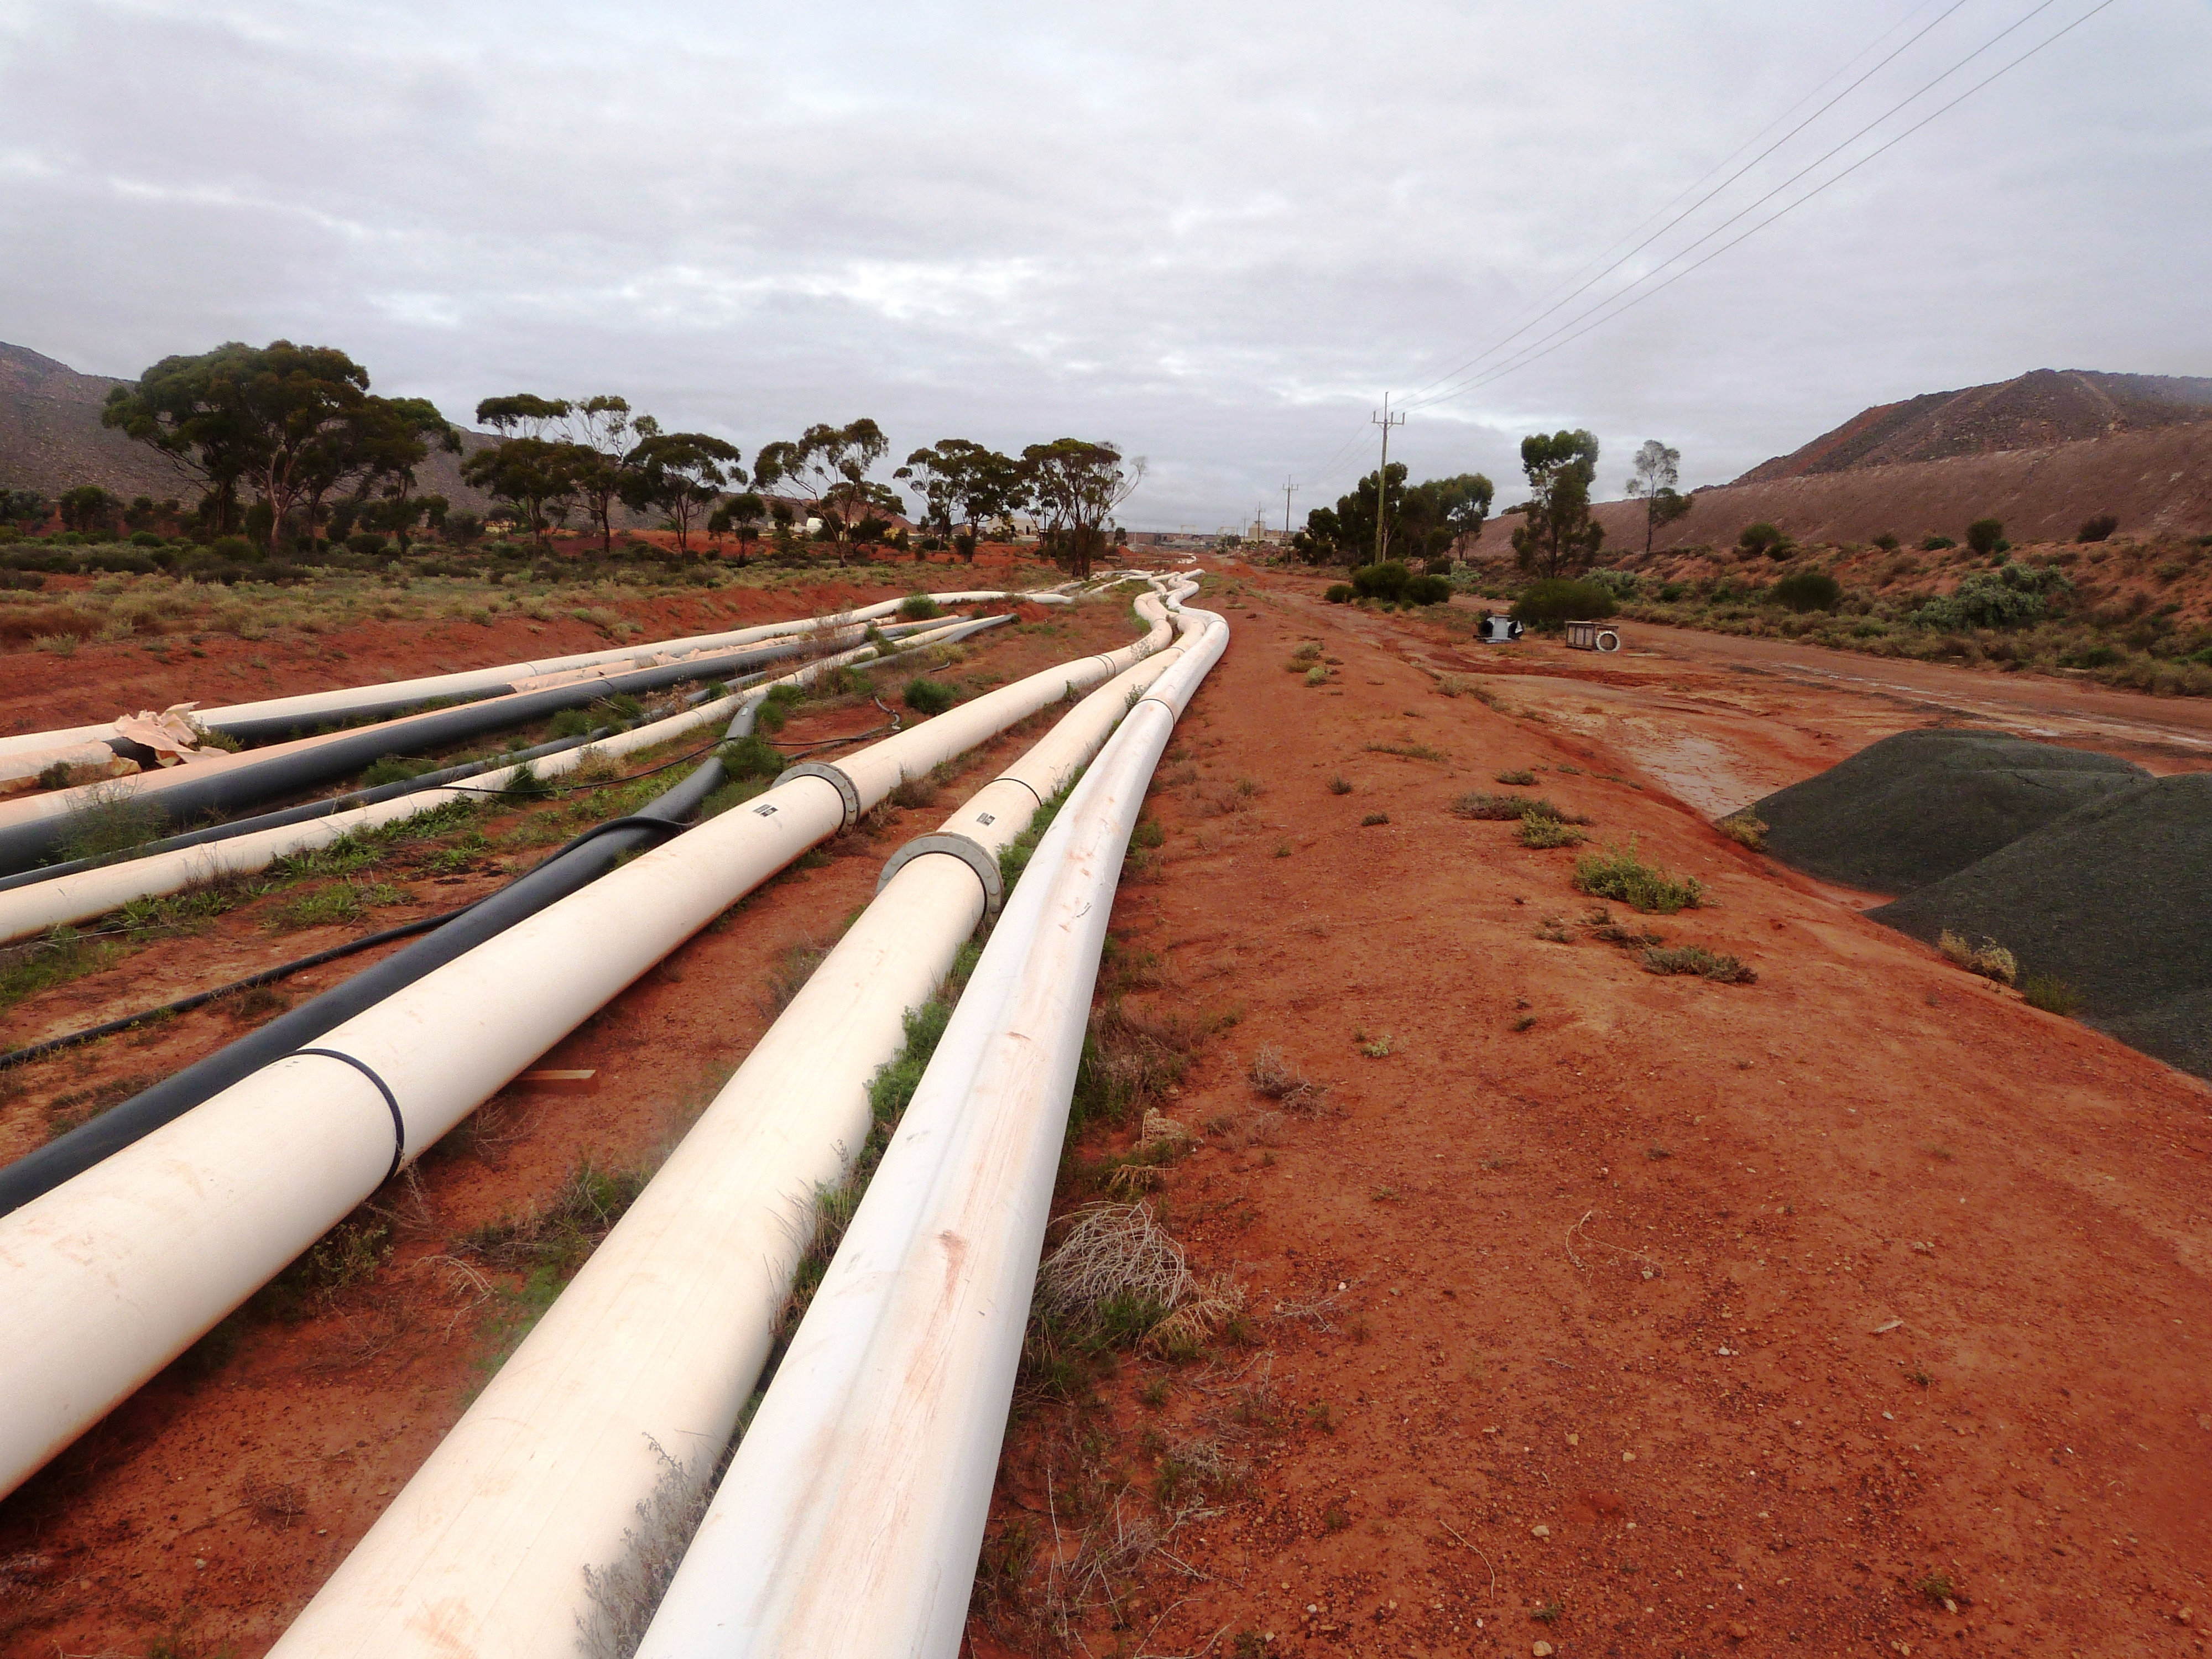
\includegraphics[width=5cm]{intro/pipeline}
\end{figure}

{\figsource{Wikipedia:  pipeline}}

\end{frame}


%%%%%%%%%%%%%%%%%%%%%%%%%%%%%%%%%%%%%%%%%%%%%%%%%%%
\begin{frame}

\frametitle{Overview}

\begin{figure}
  \centering
  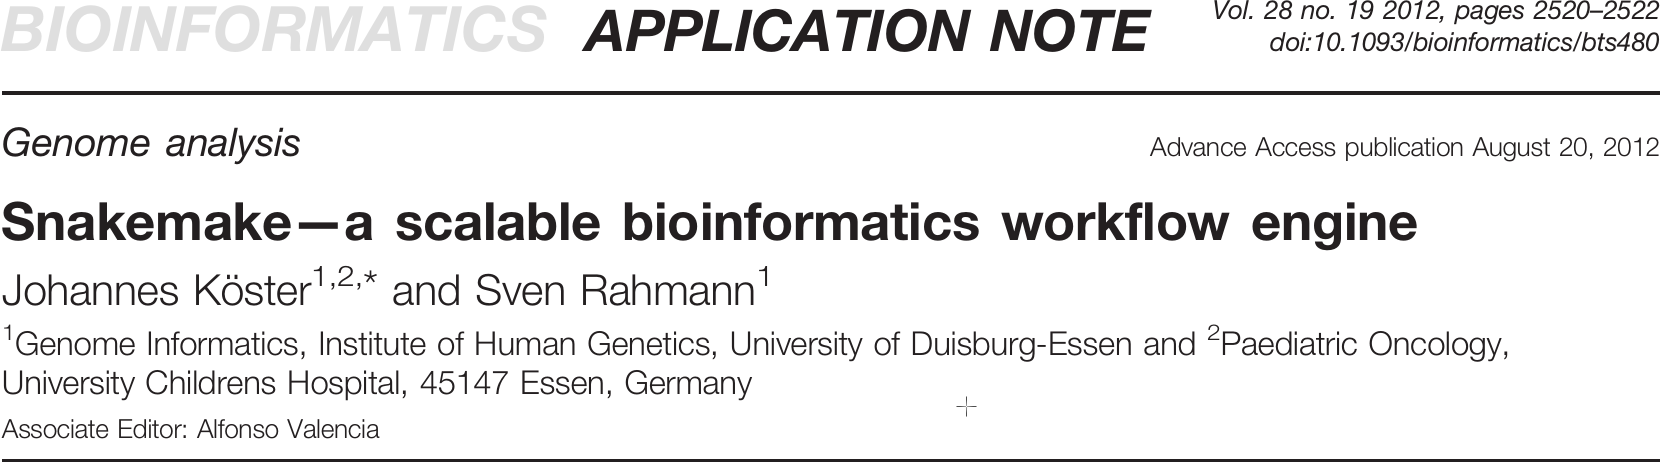
\includegraphics[width=\linewidth]{intro/kr12-bio-cover}
\end{figure}

\pause

\begin{figure}
  \centering
  {\fbox{
\includegraphics[width=8cm]{intro/snakemake-citations}}}
\end{figure}

\figsource{\citep{kr12:bio}}

\end{frame}


%%%%%%%%%%%%%%%%%%%%%%%%%%%%%%%%%%%%%%%%%%%%%%%%%%%
\begin{frame}

\frametitle{Overview}

Currently, Snakemake developers encouraging citing this ``rolling'' publication:
\begin{figure}
  \centering
  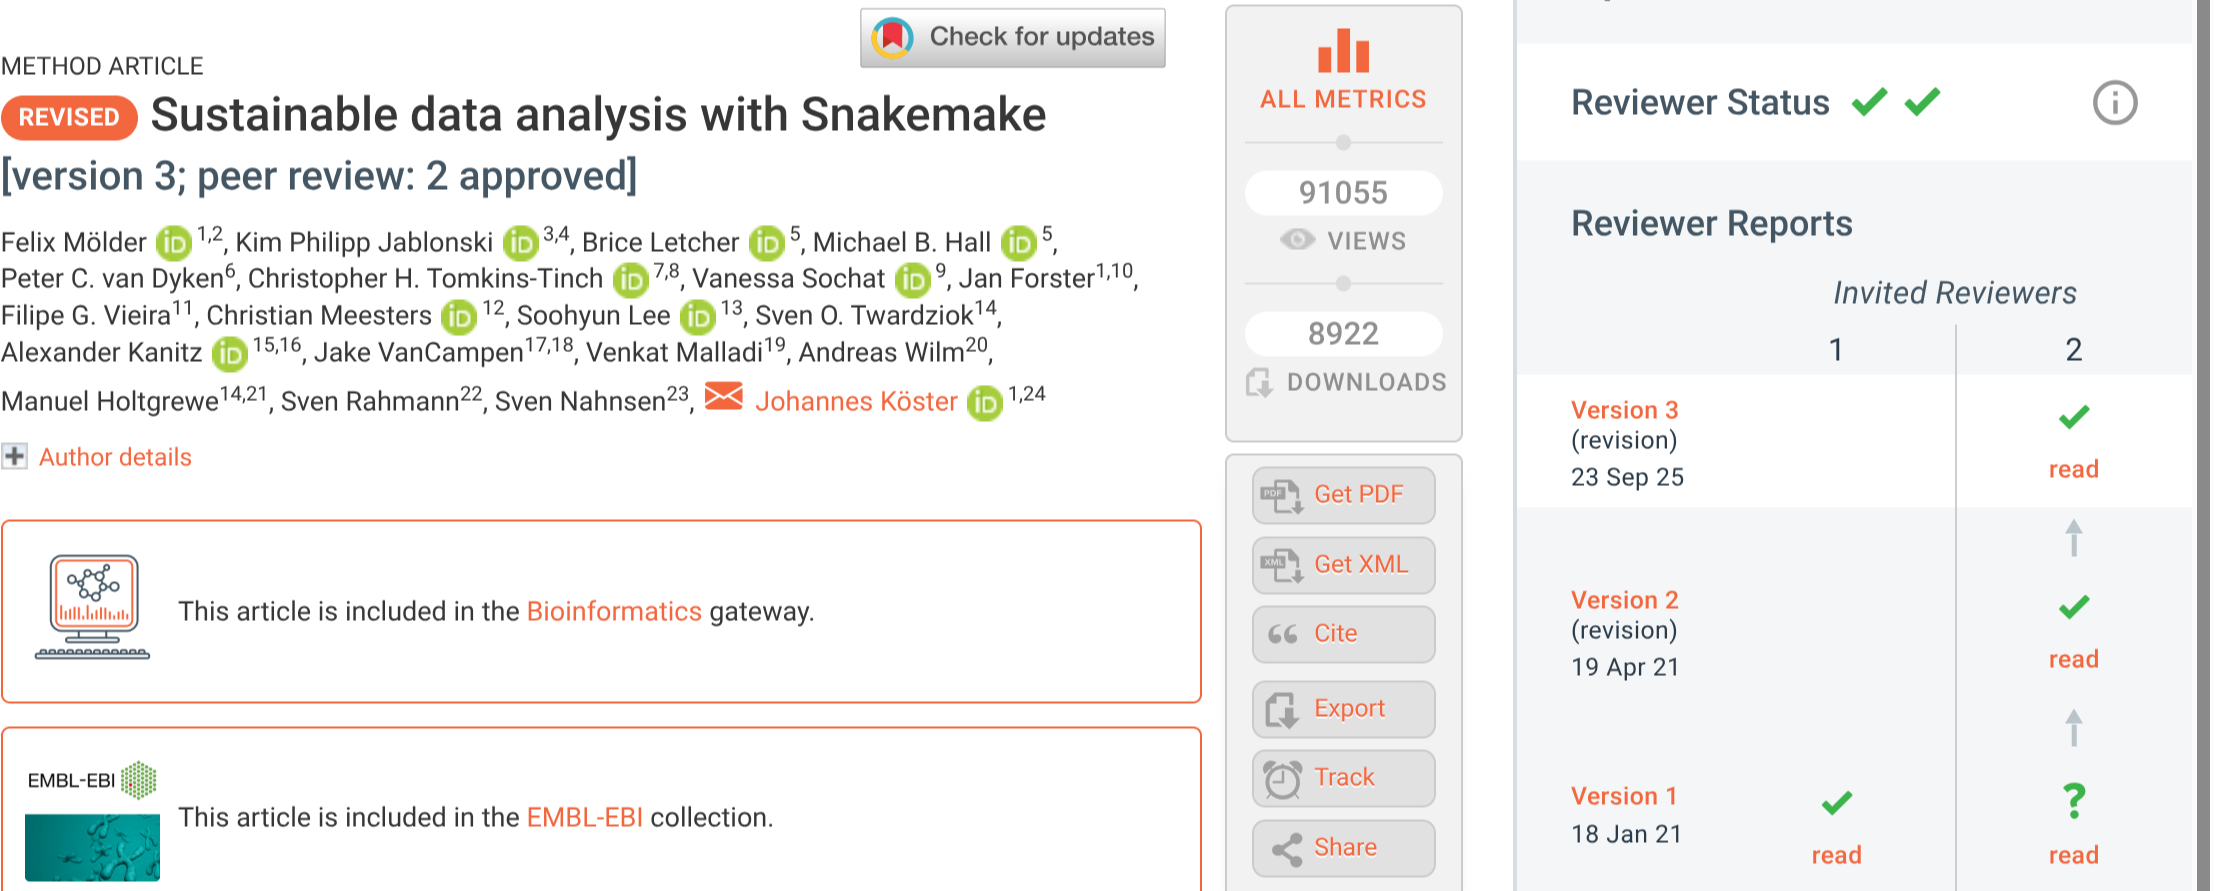
\includegraphics[width=\linewidth]{intro/mjlhv25-f1000-cover}
\end{figure}

\figsource{\citep{mjlhv25:f1000}}

\end{frame}


%%%%%%%%%%%%%%%%%%%%%%%%%%%%%%%%%%%%%%%%%%%%%%%%%%%
\begin{frame}

\frametitle{Snakemake's homepage}

\begin{figure}
  \centering
  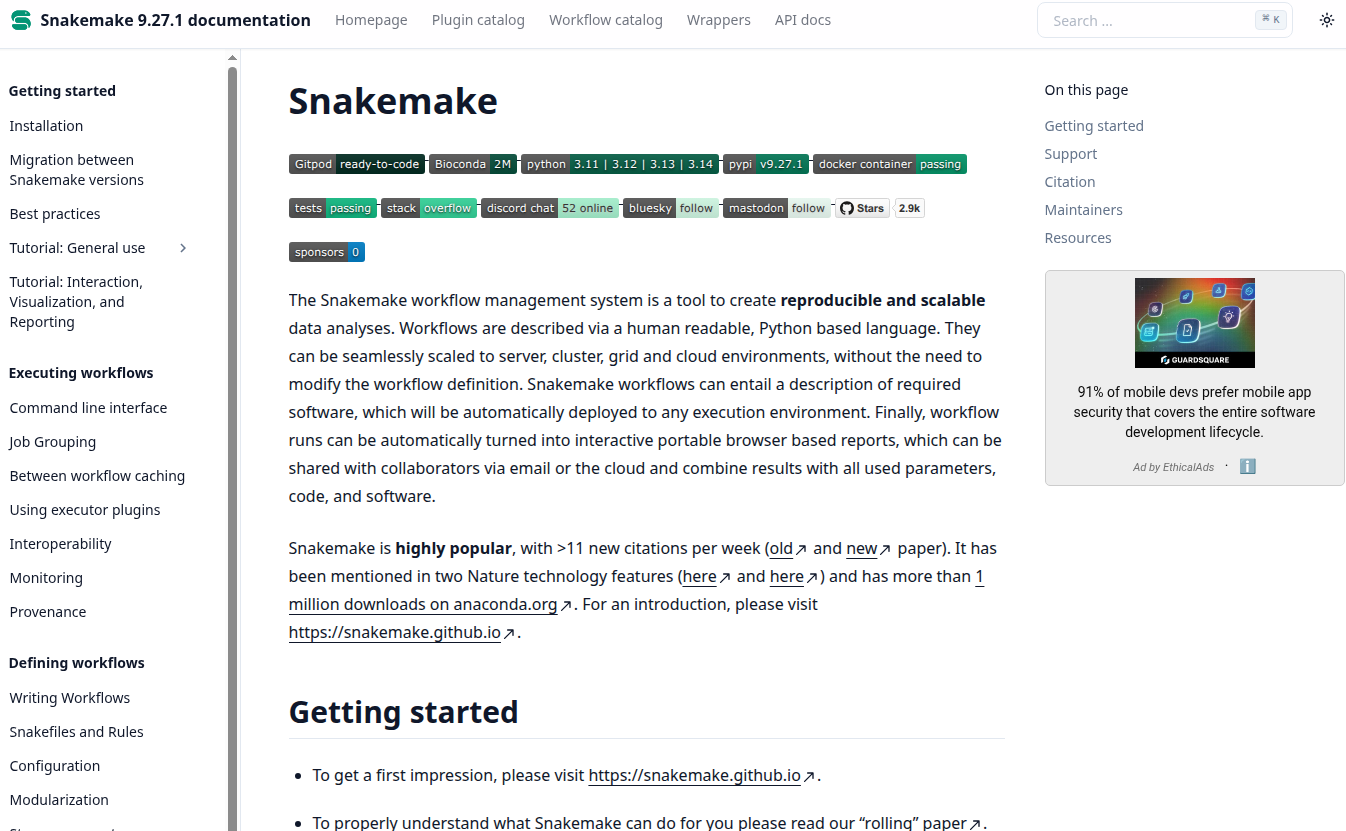
\includegraphics[height=6cm]{intro/snakemake-homepage}
\end{figure}

{\figsource{\href{https://snakemake.readthedocs.io/en/stable/}{https://snakemake.readthedocs.io/en/stable/}}}

\end{frame}


%%%%%%%%%%%%%%%%%%%%%%%%%%%%%%%%%%%%%%%%%%%%%%%%%%%
\begin{frame}

\frametitle{Snakemake's tutorial}

\begin{figure}
  \centering
  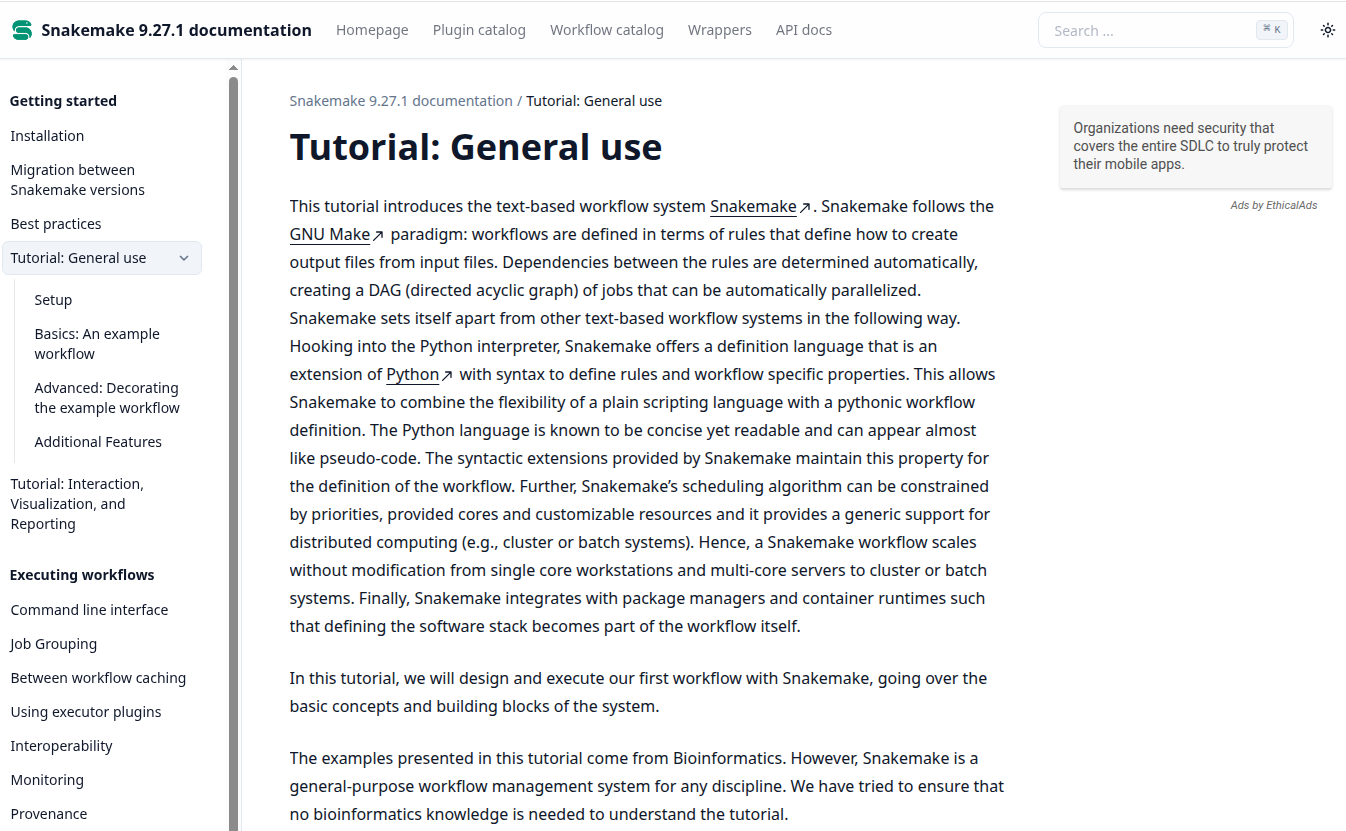
\includegraphics[height=6cm]{intro/snakemake-tutorial}
\end{figure}

{\figsource{\href{https://snakemake.readthedocs.io/en/stable/tutorial/tutorial.html}{https://snakemake.readthedocs.io/en/stable/tutorial/tutorial.html}}}

\end{frame}


%%%%%%%%%%%%%%%%%%%%%%%%%%%%%%%%%%%%%%%%%%%%%%%%%%%
\begin{frame}

\frametitle{YouTube videos}

\begin{figure}
  \centering
  {\fbox{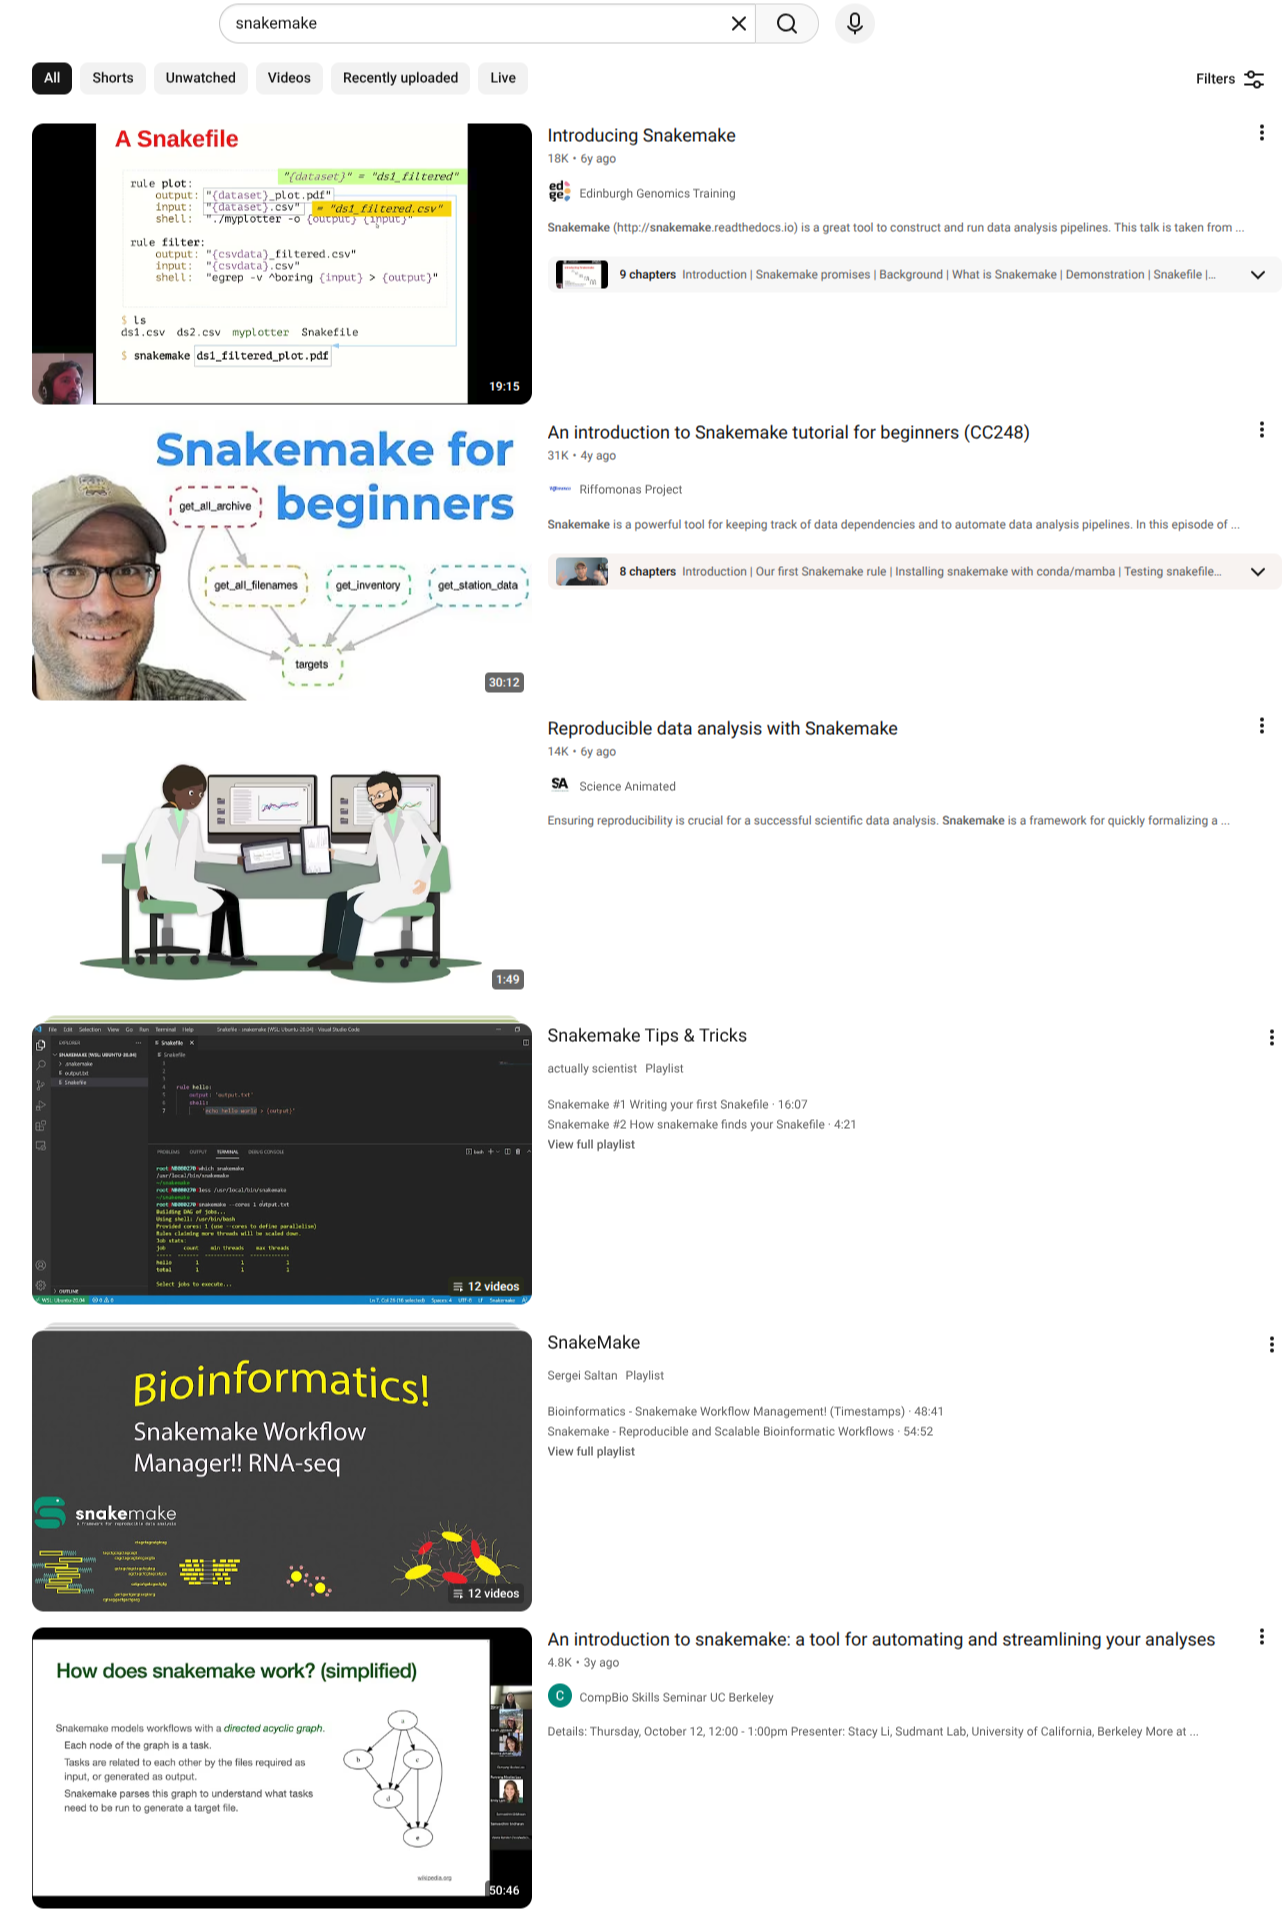
\includegraphics[height=5cm]{intro/youtube}}}
\end{figure}

So, a lot of information on the Internet now...

\end{frame}


%%%%%%%%%%%%%%%%%%%%%%%%%%%%%%%%%%%%%%%%%%%%%%%%%%%
\begin{frame}

\frametitle{My story}

By 2016, I had been working in bioinformatics for $>$10 years...
\begin{itemize}
  \item Quite stuck in my ways for workflows (i.e., {\texttt{bash}} scripts).
  \item A new colleague joined our lab with a background in CS.  Asked me where to start.  I had recently came across the Snakemake paper and gave it to him since he also knew Python.
  \item A fast learner, he picked it up in a week.  And he kept telling me how great it was.
  \item Months later, I switched, spending just over a week changing what I had been doing from {\texttt{bash}} to Snakemake.
\end{itemize}

Of course, one of the best decisions I have made as a bioinformatician...

\end{frame}


%%%%%%%%%%%%%%%%%%%%%%%%%%%%%%%%%%%%%%%%%%%%%%%%%%%
\begin{frame}

\frametitle{Talk's motivation}

Motivation of this talk:
\begin{itemize}
  \item I assume that you have a workflow / need to develop a workflow.
  \item There are so many languages and tools out there... \Smiles{-1.0}
  \item You are wondering if Snakemake is ``worth your time''...
\end{itemize}
\vs

Everything might be too fast today.  My aim is to provide a ``bird's eye'' view so that (hopefully) you have enough information to decide if you should invest more time.
\vs

If it is what you are looking for, then you have the Snakemake homepage, YouTube videos, etc. as your next resource.

\end{frame}


%%%%%%%%%%%%%%%%%%%%%%%%%%%%%%%%%%%%%%%%%%%%%%%%%%%
\begin{frame}

\frametitle{Talk's motivation}

``Disclaimer'':
\begin{itemize}
  \item Despite using it for 10 years, I only know what I needed.  I have not yet explored many (newer...) features about Snakemake.
  \item Have been happy with it since 2016; did not look into alternatives.  No doubt there are better alternatives out there!
\end{itemize}
\vs

Alternatives:
\begin{itemize}
  \item NextFlow
  \item Common Workflow Language (CWL)
  \item Galaxy (i.e., web browser based)
\end{itemize}

\end{frame}


%%%%%%%%%%%%%%%%%%%%%%%%%%%%%%%%%%%%%%%%%%%%%%%%%%%
\begin{frame}

\frametitle{Google trends}

\begin{figure}
  \centering
  {\fbox{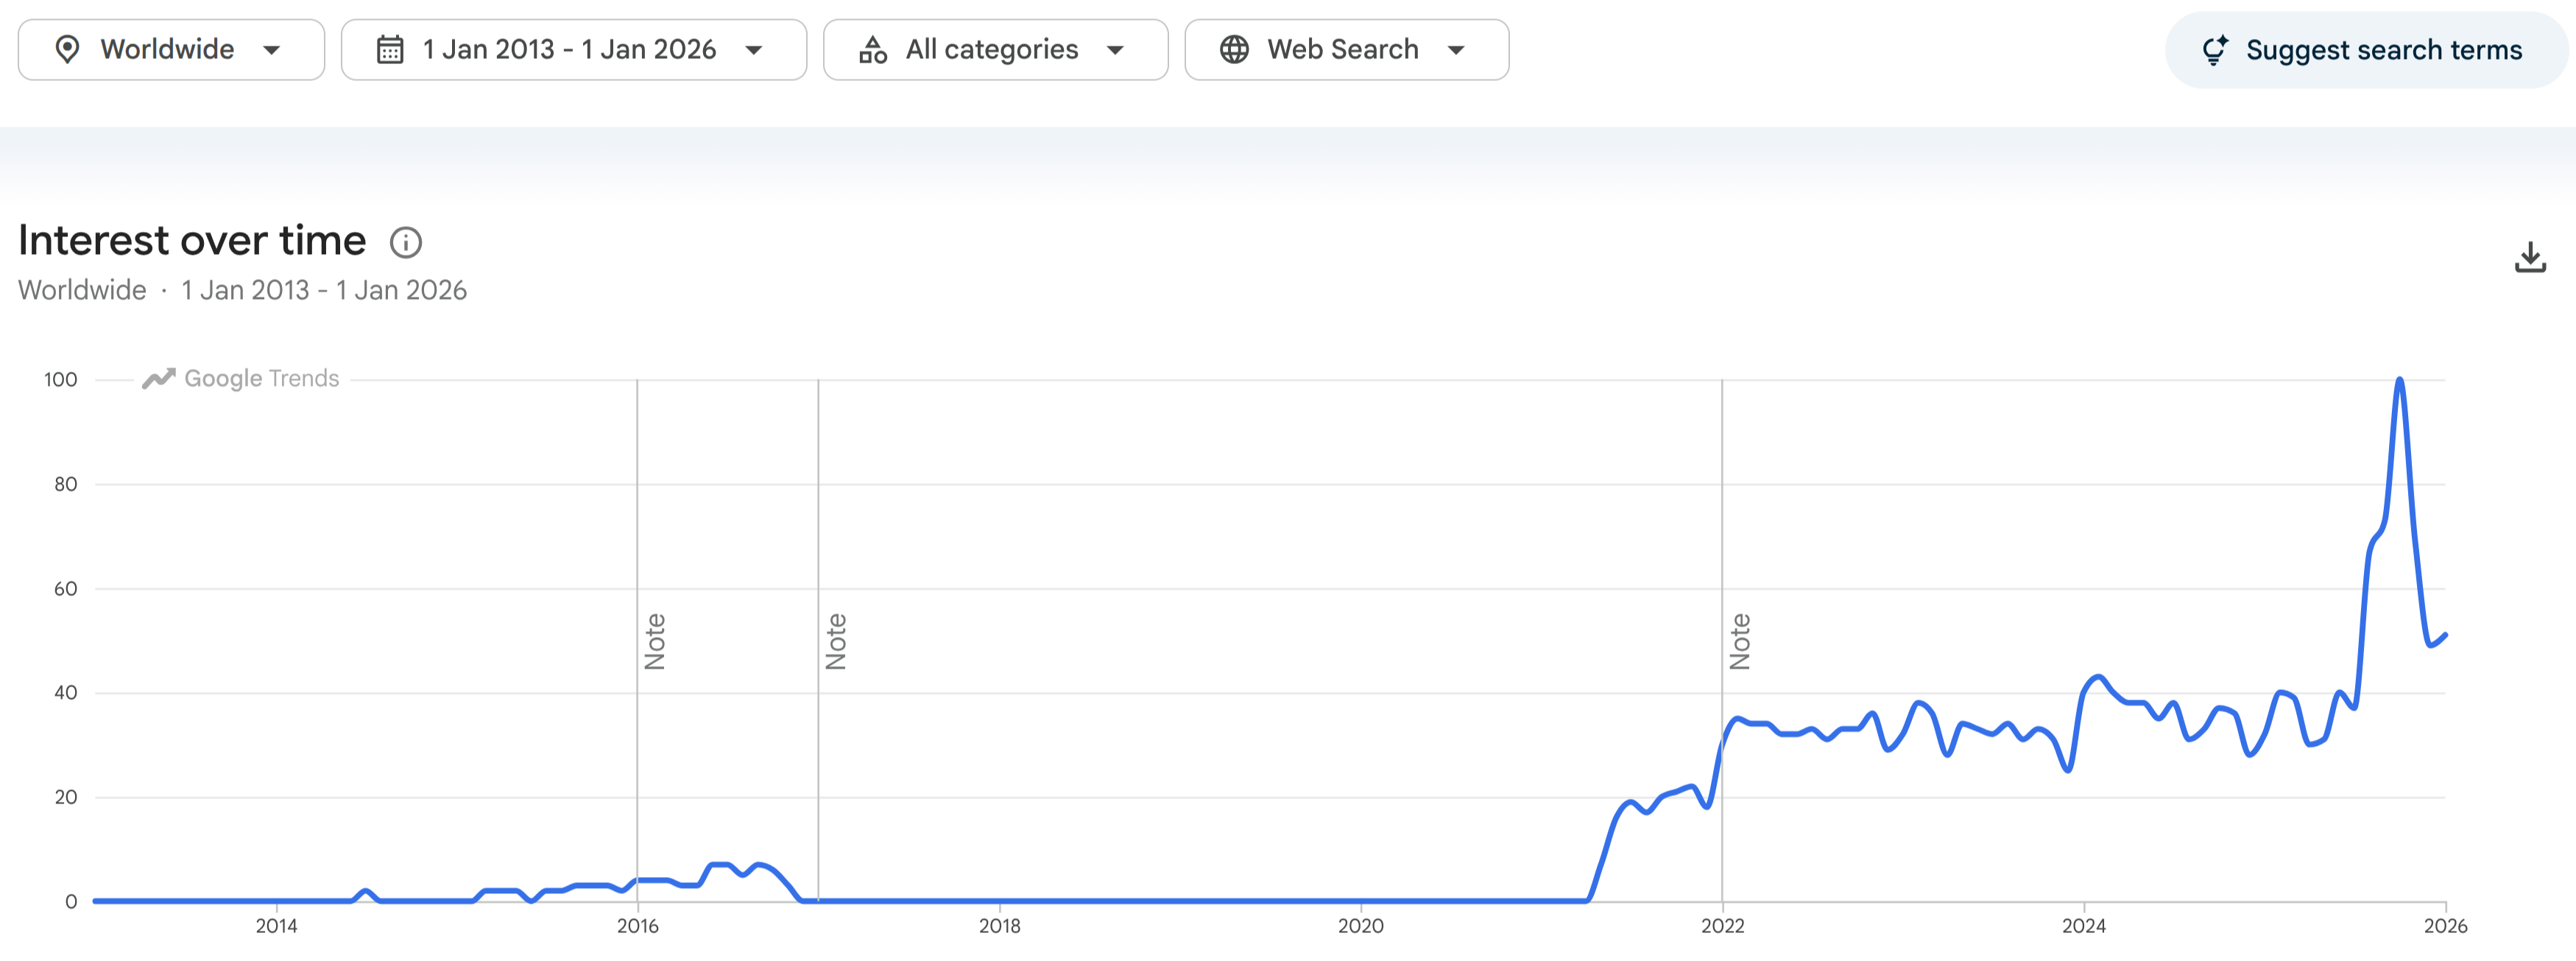
\includegraphics[width=\linewidth]{intro/google-trends}}}
\end{figure}

\end{frame}


%%%%%%%%%%%%%%%%%%%%%%%%%%%%%%%%%%%%%%%%%%%%%%%%%%%
\begin{frame}

\frametitle{Overview}

\begin{itemize}
  \item Background to the problem
  \item Basic structure of Snakemake files through working examples
  \item A final ``larger'' example
  \item Some random tips
  \item Summary
    \begin{itemize}
      \item Answers to questions that people have asked me before
    \end{itemize}
\end{itemize}
\vs

If you find these slides useful (or if I am talking too fast...), my last slide has a QR code to these PDF slides.

\end{frame}





%%%%%%%%%%%%%%%%%%%%%%%%%%%%%%%%%%%%%%%%%%%%%%%%
%%%%%%%%%%%%%%%%%%%%%%%%%%%%%%%%%%%%%%%%%%%%%%%%
\section{Background}


%%%%%%%%%%%%%%%%%%%%%%%%%%%%%%%%%%%%%%%%%%%%%%%%%%%
\begin{frame}

\frametitle{Pipeline}

Sequence of programs, running one after the other:
\begin{figure}
  \centering
  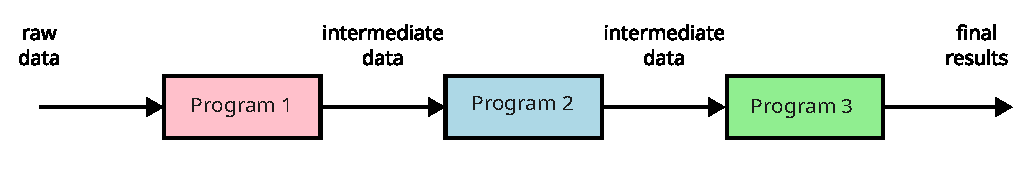
\includegraphics[width=\linewidth]{background/pipeline-example-straight.eps}
\end{figure}

\end{frame}


%%%%%%%%%%%%%%%%%%%%%%%%%%%%%%%%%%%%%%%%%%%%%%%%%%%
\begin{frame}

\frametitle{Pipeline}

Branching is also possible:
\begin{figure}
  \centering
  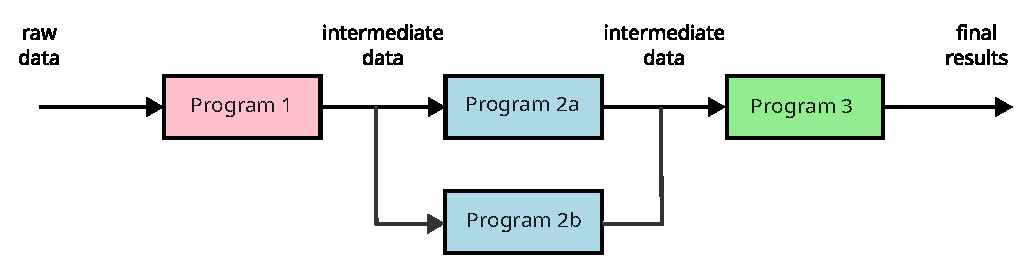
\includegraphics[width=\linewidth]{background/pipeline-example-branching.eps}
\end{figure}

\end{frame}


%%%%%%%%%%%%%%%%%%%%%%%%%%%%%%%%%%%%%%%%%%%%%%%%%%%
\begin{frame}

\frametitle{Counting characters}

Running a sequence of programs is not new to bioinformatics.
\vs

Suppose we wanted to count the number of words and characters in the first 1000 lines of the file {\texttt{alice29}}.
\vs

In Linux, we can do the following with a temporary file:
\begin{small}
\begin{table}
  \begin{tabular}{l}
  {\texttt{head -n 1000 alice29 {\textgreater}tmp1.txt}} \\
  {\texttt{wc -w -c tmp1.txt {\textgreater}alice29.count}} \\
  \end{tabular}
\end{table}
\end{small}
\vs

\pause

Or, we can use the vertical bar or ``pipe'' character (\textbar) as follows:
\begin{small}
\begin{table}
  \begin{tabular}{l}
  {\texttt{cat alice29 {\textbar} head -n 1000 {\textbar} wc -w -c {\textgreater}alice29.count}} \\
  \end{tabular}
\end{table}
\end{small}

\end{frame}


%%%%%%%%%%%%%%%%%%%%%%%%%%%%%%%%%%%%%%%%%%%%%%%%%%%
\begin{frame}

\frametitle{Make}

The program {\texttt{Make}} takes this one step further by allowing users to manage {\magenta{dependencies}}.
\vs

A file called {\texttt{Makefile}} is read by {\texttt{Make}}.
\vs

It can indicate that {\texttt{alice29.count}} is updated only if {\texttt{alice29}} was updated.

\end{frame}


%%%%%%%%%%%%%%%%%%%%%%%%%%%%%%%%%%%%%%%%%%%%%%%%%%%
\begin{frame}

\frametitle{Make}

\begin{figure}
  \centering
  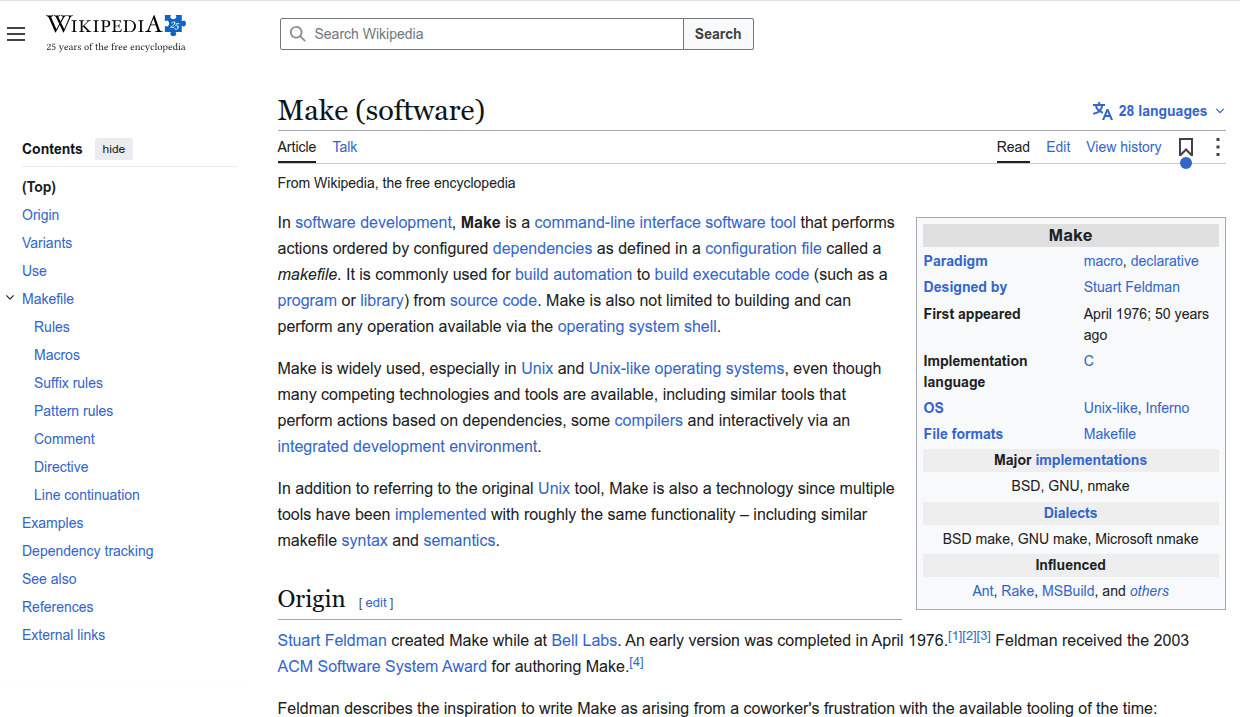
\includegraphics[width=\linewidth]{background/make-wikipedia}
\end{figure}

\end{frame}


%%%%%%%%%%%%%%%%%%%%%%%%%%%%%%%%%%%%%%%%%%%%%%%%%%%
\begin{frame}

\frametitle{Makefile}

Typically, a {\texttt{Makefile}} has a series of rules.  One rule looks like this:
\vs

\begin{figure}
  \centering
  {\fbox{
  \begin{tabular}{l}
\texttt{target:  prerequisites}\\
\texttt{{\D\D}command}\\
\texttt{{\D\D}$\vdots$}\\
\texttt{{\D\D}command}\\
  \end{tabular}
  }}
\end{figure}
\vs

{\red{$\rightarrow$}} If the dates of the files in the {\blue{prerequisites}} are newer than the {\green{target}}, then update the target by running the {\magenta{commands}} (which are preceded by a single tab character).

\end{frame}


%%%%%%%%%%%%%%%%%%%%%%%%%%%%%%%%%%%%%%%%%%%%%%%%%%%
\begin{frame}

\frametitle{``Make'' example}

As a series of commands:
\begin{scriptsize}
\begin{figure}
  \centering
  {\fbox{
  \begin{tabular}{l}
{\texttt{alice29.count:  alice29}} \\
{\D\D}{\texttt{head -n 1000 alice29 {\textgreater}tmp1.txt}} \\
{\D\D}{\texttt{wc -w -c tmp1.txt {\textgreater}alice29.count}} \\
  \end{tabular}
  }}
\end{figure}
\end{scriptsize}

\pause

As one long command with pipes:
\begin{scriptsize}
\begin{figure}
  \centering
  {\fbox{
  \begin{tabular}{l}
{\texttt{alice29.count:  alice29}} \\
{\D\D}{\texttt{cat alice29 {\textbar} head -n 1000 {\textbar} wc -w -c {\textgreater}alice29.count}} \\
  \end{tabular}
  }}
\end{figure}
\end{scriptsize}

\end{frame}


%%%%%%%%%%%%%%%%%%%%%%%%%%%%%%%%%%%%%%%%%%%%%%%%%%%
\begin{frame}

\frametitle{``Make'' example\footnote{V1}}

\begin{figure}
  \centering
  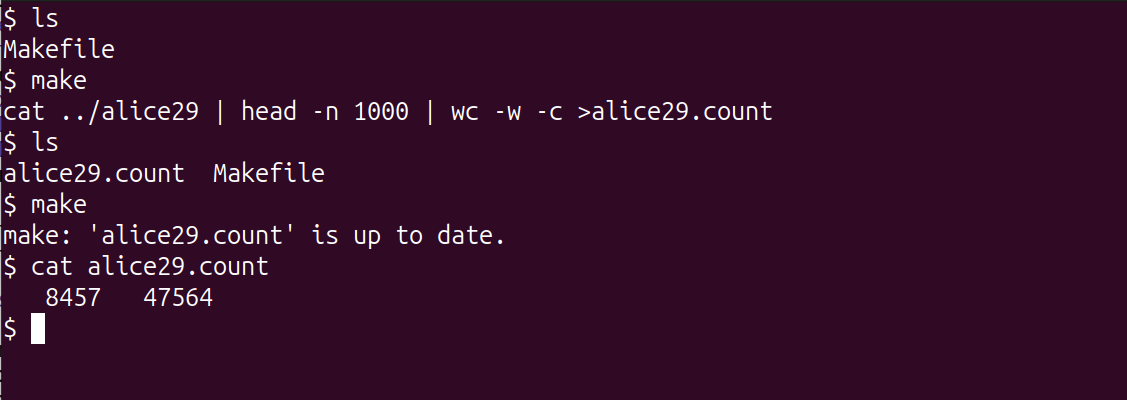
\includegraphics[width=\linewidth]{background/example-v1}
\end{figure}

\end{frame}


%%%%%%%%%%%%%%%%%%%%%%%%%%%%%%%%%%%%%%%%%%%%%%%%%%%
\begin{frame}

\frametitle{``Make'' now}

Make and Makefiles have not disappeared:
\begin{itemize}
  \item The ``make'' program still exists; and to keep something trivial up-to-date, it remains very useful.
\end{itemize}
\vs

Many similar tools have since existed that have ``Make'' in their names:
\begin{itemize}
  \item CMake
  \item qmake
  \item Snakemake
\end{itemize}

\end{frame}


%%%%%%%%%%%%%%%%%%%%%%%%%%%%%%%%%%%%%%%%%%%%%%%%%%%
\begin{frame}

\frametitle{Make}

Their purposes:
\begin{itemize}
  \item CMake -- Cross-platform make, for projects made with C/C++ (for example)
  \item qmake -- Qt projects make, for C++ projects using Qt to make a graphical user interface
  \item Snakemake -- Development of workflows with Python syntax
\end{itemize}

\end{frame}


%%%%%%%%%%%%%%%%%%%%%%%%%%%%%%%%%%%%%%%%%%%%%%%%%%%
\begin{frame}

\frametitle{Snakemake}

So, that is where the ``make'' part of Snake{\green{make}} comes from!
\vs

The ``Snake'' part is due to {\blue{Snake}}make being made with Python and borrows some of Python's syntax.
\vs

But it is a separate program with a different file format.  i.e., Snakemake files are not Python programs.

\end{frame}


%%%%%%%%%%%%%%%%%%%%%%%%%%%%%%%%%%%%%%%%%%%%%%%%%%%%%%%
\begin{frame}

\frametitle{Data sets}

Two sets of text files will be considered.  Both are used to test text compression systems (i.e., my former area of research):
\begin{itemize}
  \item Calgary corpus from the University of Calgary \citep{bcw90:book}.
  \item Canterbury corpus from the University of Canterbury \citep{ab97:dcc}.
\end{itemize}
\vs

While not bioinformatics related, we are all familiar with text and both are publicly available.
\vs

Even so, I have taken only the first 1,024 lines of each since the originals are too large for our purposes.

\end{frame}





%%%%%%%%%%%%%%%%%%%%%%%%%%%%%%%%%%%%%%%%%%%%%%%%
%%%%%%%%%%%%%%%%%%%%%%%%%%%%%%%%%%%%%%%%%%%%%%%%
\section{Basic structure}


%%%%%%%%%%%%%%%%%%%%%%%%%%%%%%%%%%%%%%%%%%%%%%%%%%%%%%%
\begin{frame}

\frametitle{Basic format}

Like Make, a Snakemake file consists of a series of rules
\begin{itemize}
  \item While the format is different from Make, each rule has:
    \begin{itemize}
      \item A name
      \item Series of directives:
      \begin{enumerate}
        \item Input(s)
        \item Output(s)
        \item Command(s) to run to convert the inputs to the outputs
        \item ...
      \end{enumerate}
    \end{itemize}
  \item Rules can be chained together and/or create branches.
  \item A rule is applied if the date/time of the input(s) is newer than the output(s).
\end{itemize}

\end{frame}


%%%%%%%%%%%%%%%%%%%%%%%%%%%%%%%%%%%%%%%%%%%%%%%%%%%%%%%
\begin{frame}

\frametitle{Snakemake program}

The program is simply {\texttt{snakemake}}.
\vs

If the program is not installed on the machine you are using, then see the documentation on how to install it.
\vs

If you administer your own Linux machine, then you can install it with just {\texttt{sudo apt-get install snakemake}}.
\vs

Ubuntu 26.04 LTS will install version 7.32.4.  The latest version appears to be 9.27.1.

\end{frame}


%%%%%%%%%%%%%%%%%%%%%%%%%%%%%%%%%%%%%%%%%%%%%%%%%%%%%%%
\begin{frame}

\frametitle{Filename}

Like {\texttt{Make}}, when you run {\texttt{snakemake}}, it will search for a file of rules.  This file should be one of the following:
\begin{itemize}
  \item {\texttt{Snakefile}},
  \item {\texttt{snakefile}},
  \item {\texttt{workflow/Snakefile}},
  \item {\texttt{workflow/snakefile}}
\end{itemize}
\vs

{\magenta{However}}, I tend to use the {\texttt{--snakefile}} option to specify my own filename:  {\texttt{Snakefile.smk}} (so that I can find my Snakemake files easily).
\vs

Like Python scripts which can be broken up into modules and ``imported'' in, the rules in a Snakemake file can be separated into multiple files and ``included'' in.

\end{frame}


%%%%%%%%%%%%%%%%%%%%%%%%%%%%%%%%%%%%%%%%%%%%%%%%%%%%%%%
\begin{frame}

\frametitle{Snakemake options}

See the manual for a list of options.  But besides {\texttt{--snakefile}}, I find these useful:
\begin{itemize}
  \item {\texttt{--cores}} -- number of cores to use; rules that are not dependent on each other can execute in parallel across multiple cores
  \item {\texttt{--dryrun}} -- perform a ``dry run'' (i.e., do not actually run)
  \item {\texttt{-p}} -- print shell commands
\end{itemize}

\end{frame}


%%%%%%%%%%%%%%%%%%%%%%%%%%%%%%%%%%%%%%%%%%%%%%%%%%%%%%%
\begin{frame}[fragile]

\frametitle{Sample Rule\footnote{V2}}

\begin{figure}
  \centering
  \begin{tabular}{lc}
DATA\_DIR = "../../data" & \only<7>{{\red{$\leftarrow$}}} \\
OUTPUT\_DIR = "Output" & \only<7>{{\red{$\leftarrow$}}} \\
\\
rule CountAlice: & \only<1>{{\red{$\leftarrow$}}} \\
  {\D\D}input:  DATA\_DIR + "/canterbury/alice29" & \only<2>{{\red{$\leftarrow$}}} \\
  {\D\D}output:  OUTPUT\_DIR + "/alice29.count" & \only<3>{{\red{$\leftarrow$}}} \\
  {\D\D}shell: & \only<4>{{\red{$\leftarrow$}}} \\
  {\D\D\D\D}""" & \only<5>{{\red{$\leftarrow$}}} \\
  {\D\D\D\D}cat \{input\} | head -n 1000 | wc -w -c >\{output\} & \only<6>{{\red{$\leftarrow$}}} \\
  {\D\D\D\D}""" & \only<5>{{\red{$\leftarrow$}}} \\
  \end{tabular}
\end{figure}

Note:  Variables are enclosed in curly braces.

\end{frame}


%%%%%%%%%%%%%%%%%%%%%%%%%%%%%%%%%%%%%%%%%%%%%%%%%%%%%%%
\begin{frame}

\frametitle{Sample Rule\footnote{V2}}

\begin{figure}
  \centering
  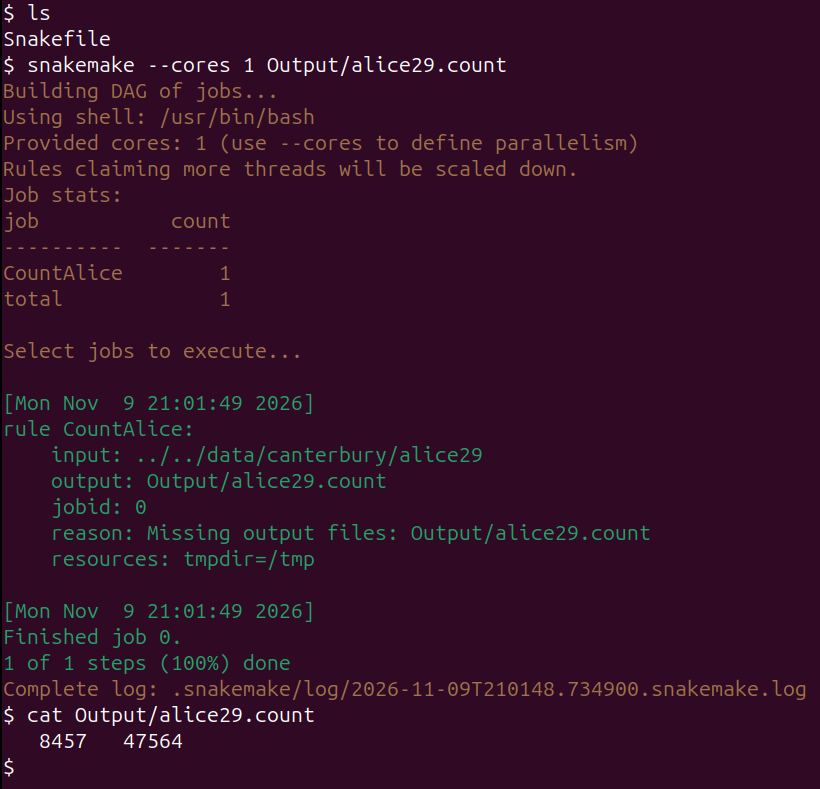
\includegraphics[height=7cm]{structure/example-v2}
\end{figure}

\end{frame}


%%%%%%%%%%%%%%%%%%%%%%%%%%%%%%%%%%%%%%%%%%%%%%%%%%%
\begin{frame}[fragile]

\frametitle{Example with two rules\footnote{V3}}

\begin{tiny}
\begin{lstlisting}[frame=single,language=bash]
DATA_DIR = "../../data"
OUTPUT_DIR = "Output"

rule TopAlice:
  input:  DATA_DIR + "/canterbury/alice29"
  output:  OUTPUT_DIR + "/01-top/alice29.head"
  shell:
    """
    head -n 1000 {input} >{output}
    """

rule CountAlice:
  input:  OUTPUT_DIR + "/01-top/alice29.head"
  output:  OUTPUT_DIR + "/02-count/alice29.count"
  shell:
    """
    wc -w -c {input} >{output}
    """
\end{lstlisting}
\end{tiny}

\end{frame}


%%%%%%%%%%%%%%%%%%%%%%%%%%%%%%%%%%%%%%%%%%%%%%%%%%%%%%%
\begin{frame}

\frametitle{Sample Rule\footnote{V3}}

\begin{figure}
  \centering
  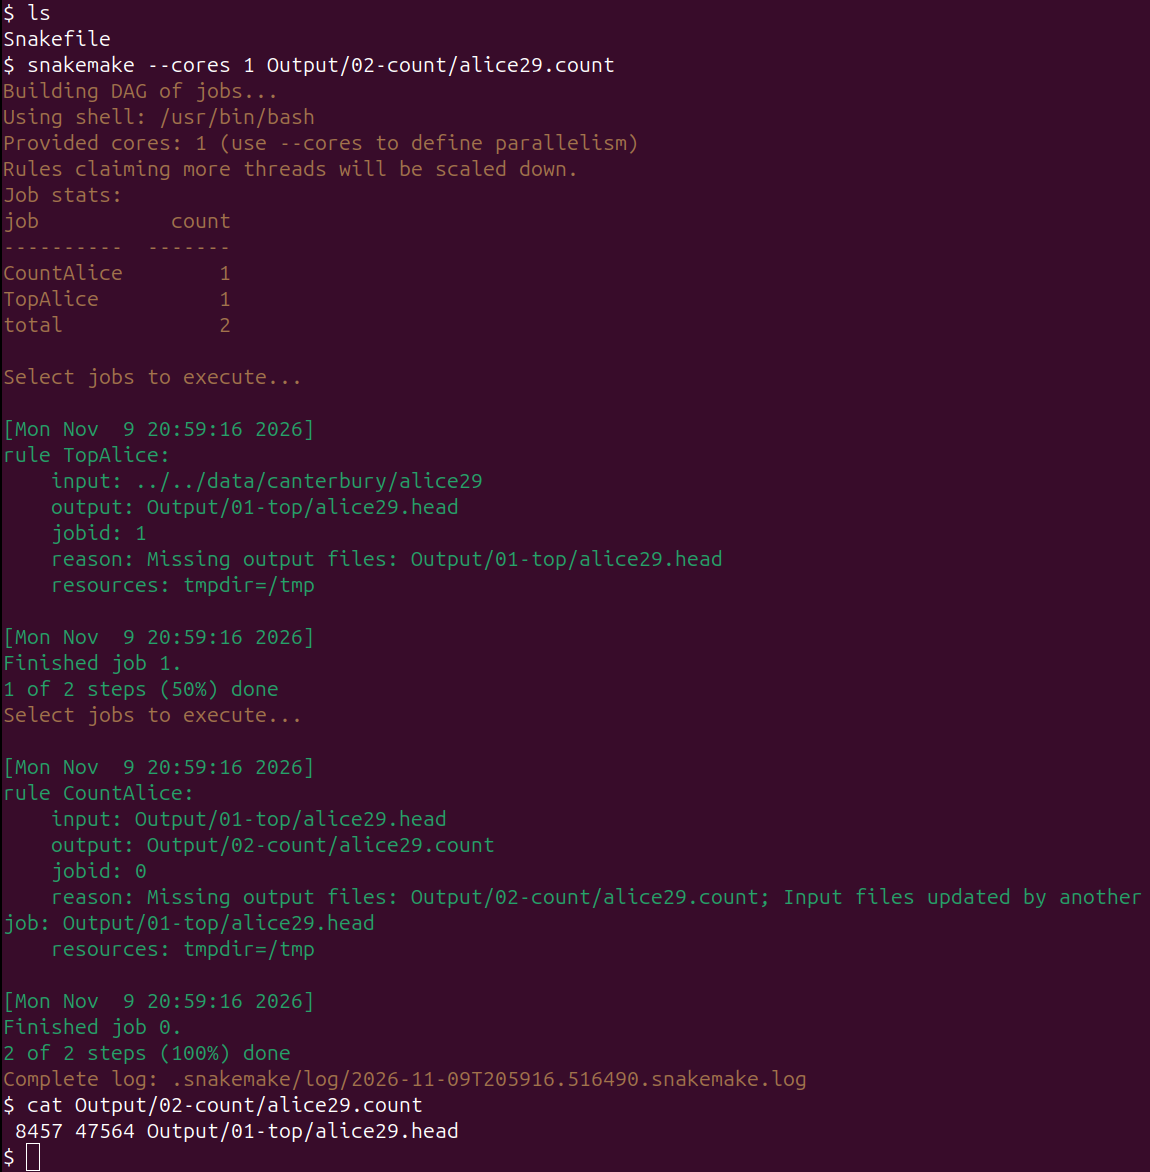
\includegraphics[height=7cm]{structure/example-v3}
\end{figure}

\end{frame}


%%%%%%%%%%%%%%%%%%%%%%%%%%%%%%%%%%%%%%%%%%%%%%%%%%%
\begin{frame}[fragile]

\frametitle{Generalising\footnote{V4}}

\begin{tiny}
\begin{lstlisting}[frame=single,language=bash]
##  Include important variables
include:  "global-vars.smk"

rule all:
  input:
    OUTPUT_DIR + "/02-count/alice29.count",
    OUTPUT_DIR + "/02-count/asyoulik.count",
    OUTPUT_DIR + "/02-count/lcet10.count",
    OUTPUT_DIR + "/02-count/plrabn12.count"

rule FileTop:
  input:  DATA_DIR + "/canterbury/{fn}"
  output:  OUTPUT_DIR + "/01-top/{fn}.head"
  shell:
    """
    head -n 1000 {input} >{output}
    """

rule Count:
  input:  OUTPUT_DIR + "/01-top/{fn}.head"
  output:  OUTPUT_DIR + "/02-count/{fn}.count"
  shell:
    """
    wc -w -c {input} >{output}
    """
\end{lstlisting}
\end{tiny}

\end{frame}


%%%%%%%%%%%%%%%%%%%%%%%%%%%%%%%%%%%%%%%%%%%%%%%%%%%
\begin{frame}[fragile]

\frametitle{Generalising\footnote{V4}}

In this example,
\begin{itemize}
  \item The path variables have been moved to a separate file called {\texttt{global-vars.smk}}.  That file has been included in.
  \item There is an {\magenta{all}} rule which has an input directive but no output directive.
    \begin{itemize}
      \item If it is first in the file, then it will be applied if you run Snakemake with no options.  (i.e., a ``default'' rule)
      \item Other rules can occur before it if they are included in (i.e., not before it in the same file).
    \end{itemize}
  \item Together, we can now process all four files by {\green{just}} adding them to the {\magenta{all}} rule.
\end{itemize}

\end{frame}



%%%%%%%%%%%%%%%%%%%%%%%%%%%%%%%%%%%%%%%%%%%%%%%%%%%%%%%
\begin{frame}

\frametitle{Generalising Results\footnote{V4}}

\begin{figure}
  \centering
  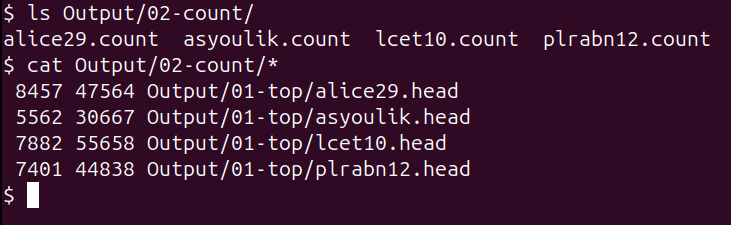
\includegraphics[width=9cm]{structure/example-v4}
\end{figure}

\end{frame}


%%%%%%%%%%%%%%%%%%%%%%%%%%%%%%%%%%%%%%%%%%%%%%%%%%%%%%%
\begin{frame}[fragile]

\frametitle{Visualisation\footnote{V4}}

Create a ``DAG'' (directed acyclic graph) for {\texttt{graphviz}} (not part of Snakemake):
\begin{tiny}
\begin{lstlisting}[frame=single,language=bash]
snakemake --cores 1 --dag | dot -Teps >dag.eps
\end{lstlisting}
\end{tiny}

\begin{figure}
  \centering
  {\fbox{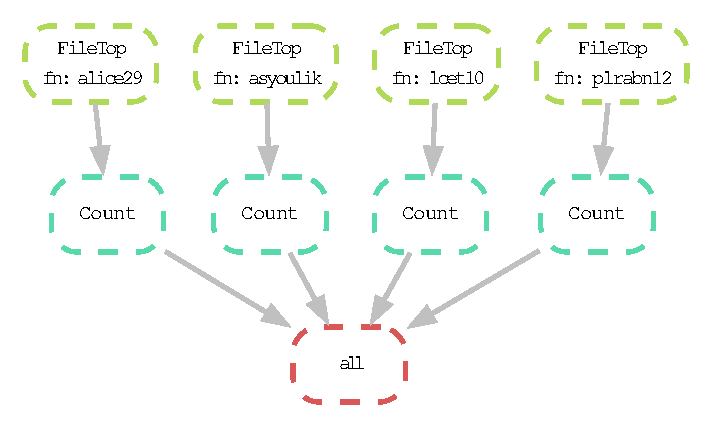
\includegraphics[width=7cm]{structure/dag-v4}}}
\end{figure}

\end{frame}


%%%%%%%%%%%%%%%%%%%%%%%%%%%%%%%%%%%%%%%%%%%%%%%%%%%%%%%
\begin{frame}[fragile]

\frametitle{Python instead of bash commands\footnote{V5}}

\begin{tiny}
\begin{lstlisting}[frame=single,language=python]
DATA_DIR = "../../data"
OUTPUT_DIR = "Output"

rule CountAlice:
  input:  DATA_DIR + "/canterbury/alice29"
  output:  OUTPUT_DIR + "/alice29.count"
  run:
    with open (output[0], "w") as outfp:
      with open (input[0]) as infp:
        num_words = 0
        num_chars = 0
        for line in infp:
          wordslist = line.split ()
          num_words = num_words + len (wordslist)
          num_chars += (sum (len (word) for word in wordslist))
      outfp.write (str (num_words))
      outfp.write ("\t")
      outfp.write (str (num_chars) + "\t" + output[0] + "\n")
\end{lstlisting}
\end{tiny}

\end{frame}





%%%%%%%%%%%%%%%%%%%%%%%%%%%%%%%%%%%%%%%%%%%%%%%%
%%%%%%%%%%%%%%%%%%%%%%%%%%%%%%%%%%%%%%%%%%%%%%%%
\section{Final example}


%%%%%%%%%%%%%%%%%%%%%%%%%%%%%%%%%%%%%%%%%%%%%%%%%%%%%%%
\begin{frame}

\frametitle{Graph}

\begin{figure}
  \centering
  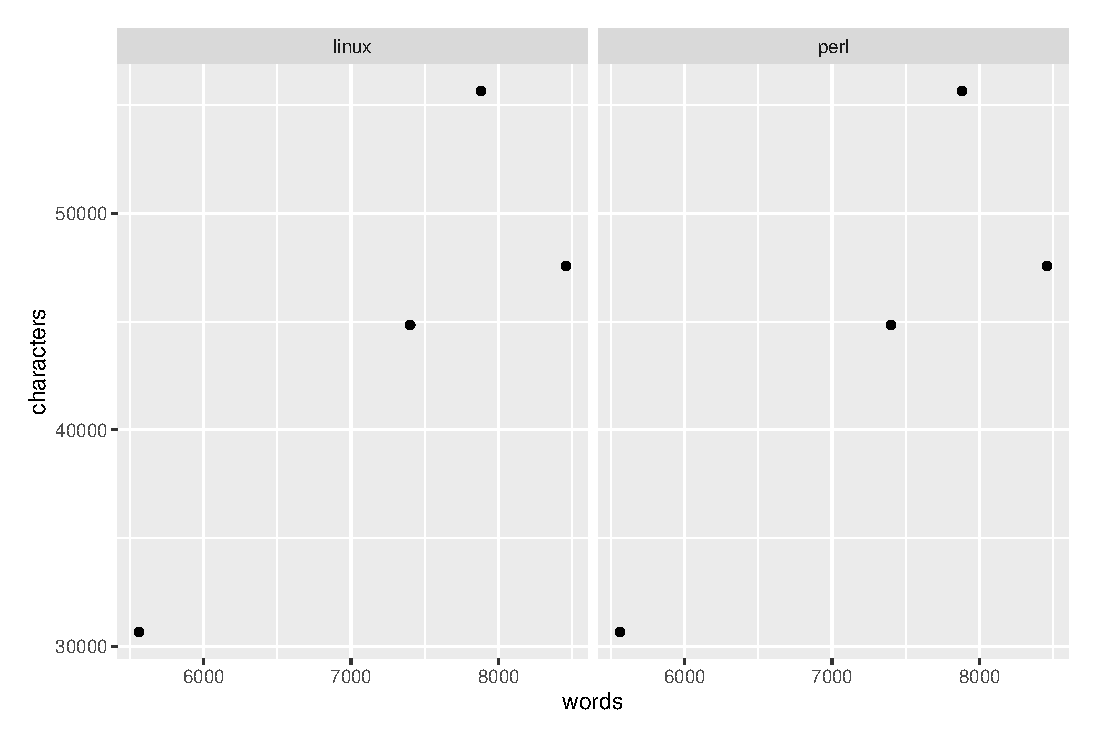
\includegraphics[width=10cm]{finalex/canterbury}
\end{figure}

\end{frame}


%%%%%%%%%%%%%%%%%%%%%%%%%%%%%%%%%%%%%%%%%%%%%%%%%%%%%%%
\begin{frame}

\frametitle{Data table}

Create a data table in tab-separated format:  {\texttt{fileslist.tsv}}.

\begin{table}
  \begin{tabular}{ccc}
  \hline
ID & corpus & filename \\
  \hline
1 & calgary & book1 \\
2 & calgary & book2 \\
3 & calgary & news \\
4 & calgary & progc \\
5 & calgary & progl \\
6 & calgary & progp \\
7 & canterbury & alice29 \\
8 & canterbury & asyoulik \\
9 & canterbury & lcet10 \\
10 & canterbury & plrabn12 \\
  \hline
  \end{tabular}
\end{table}

\end{frame}


%%%%%%%%%%%%%%%%%%%%%%%%%%%%%%%%%%%%%%%%%%%%%%%%%%%%%%%
\begin{frame}[fragile]

\frametitle{Main Snakefile\footnote{V6}}

\begin{tiny}
\begin{lstlisting}[frame=single,language=bash]
import pandas as pd

from snakemake.utils import validate, min_version

configfile: "config.yml"
validate (config, schema = "config.schema.yml")

fileslist_panda = pd.read_table (config["fileslist"], sep='\t', lineterminator='\n')
fileslist_panda.set_index ("ID", drop=False, inplace=True)
validate (fileslist_panda, schema="fileslist.schema.yml")

##  Define global constraints on wildcards
wildcard_constraints:
  corpus = "calgary|canterbury"

##  Include important variables
include:  "global-vars.smk"

include:  "single.smk"
include:  "combine.smk"
include:  "graphs.smk"

rule all:
  input:
    OUTPUT_DIR + "/05-graphs/canterbury.jpg"
\end{lstlisting}
\end{tiny}

\end{frame}


%%%%%%%%%%%%%%%%%%%%%%%%%%%%%%%%%%%%%%%%%%%%%%%%%%%%%%%
\begin{frame}[fragile]

\frametitle{{\texttt{graphs.smk}}\footnote{V6}}

\begin{tiny}
\begin{lstlisting}[frame=single,language=bash]
rule Scatterplot:
  input:
    input_fn1 = OUTPUT_DIR + "/04-combine-perl/{corpus}.tsv",
    input_fn2 = OUTPUT_DIR + "/04-combine-linux/{corpus}.tsv",
  output:
    output_fn1 = OUTPUT_DIR + "/05-graphs/{corpus}.jpg",
    output_fn2 = OUTPUT_DIR + "/05-graphs/{corpus}.png",
    output_fn3 = OUTPUT_DIR + "/05-graphs/{corpus}.eps"
  params:
    corpus = "{corpus}",
    myeps = lambda wildcards: config["my_options"]["postscript"]
  log:
    log_fn1 = OUTPUT_DIR + "/05-graphs/{corpus}.log"
  shell:
    """
    ##  {params.corpus} is available
    mypng="png"
    {TOOLS_DIR}/scatterplot.R --type jpg --perl {input.input_fn1} --linux
      {input.input_fn2} --output {output.output_fn1} >{log.log_fn1} 2>&1
    {TOOLS_DIR}/scatterplot.R --type ${{mypng}} --perl {input.input_fn1} --linux
      {input.input_fn2} --output {output.output_fn2} >>{log.log_fn1} 2>&1
    {TOOLS_DIR}/scatterplot.R --type {params.myeps} --perl {input.input_fn1} --linux
      {input.input_fn2} --output {output.output_fn3} >>{log.log_fn1} 2>&1
    """
\end{lstlisting}
\end{tiny}

\end{frame}


%%%%%%%%%%%%%%%%%%%%%%%%%%%%%%%%%%%%%%%%%%%%%%%%%%%%%%%
\begin{frame}[fragile]

\frametitle{{\texttt{combine.smk}}\footnote{V6}}

\begin{tiny}
\begin{lstlisting}[frame=single,language=bash]
rule CombinePerl:
  input:  GatherPerl
  output:  OUTPUT_DIR + "/04-combine-perl/{corpus}.tsv"
  shell:
    """
    cat {input} >{output}
    """
\end{lstlisting}
\end{tiny}

\end{frame}


%%%%%%%%%%%%%%%%%%%%%%%%%%%%%%%%%%%%%%%%%%%%%%%%%%%%%%%
\begin{frame}[fragile]

\frametitle{{\texttt{combine.smk}}\footnote{V6}}

\begin{tiny}
\begin{lstlisting}[frame=single,language=python]
def GatherPerl (wc):
  results = []  ##  Initialise empty list

  ##  Iterate through each row of the table
  for row in fileslist_panda.itertuples (index = False):
    curr_ID = str (row.ID)  ##  Convert integer to string
    curr_corpus = row.corpus  ##  Current "corpus" in this row
    curr_filename = row.filename

    ##  Check for equality between wildcard corpus and current corpus
    if wc.corpus == curr_corpus:
      d = [OUTPUT_DIR + "/02-count-perl/{f}.count".format (f=curr_filename)]
      results.extend (d)  ##  Add it to the list

  ##  Print out the results
  print (results, file=sys.stderr)

  return results
\end{lstlisting}
\end{tiny}
\pause

The {\texttt{print ()}} produces this:
\begin{tiny}
\begin{lstlisting}[frame=single,language=bash]
['Output/02-count-perl/alice29.count', 'Output/02-count-perl/asyoulik.count',
'Output/02-count-perl/lcet10.count', 'Output/02-count-perl/plrabn12.count']
\end{lstlisting}
\end{tiny}

\end{frame}


%%%%%%%%%%%%%%%%%%%%%%%%%%%%%%%%%%%%%%%%%%%%%%%%%%%%%%%
\begin{frame}[fragile]

\frametitle{Visualisation\footnote{V6}}

\begin{figure}
  \centering
  {\fbox{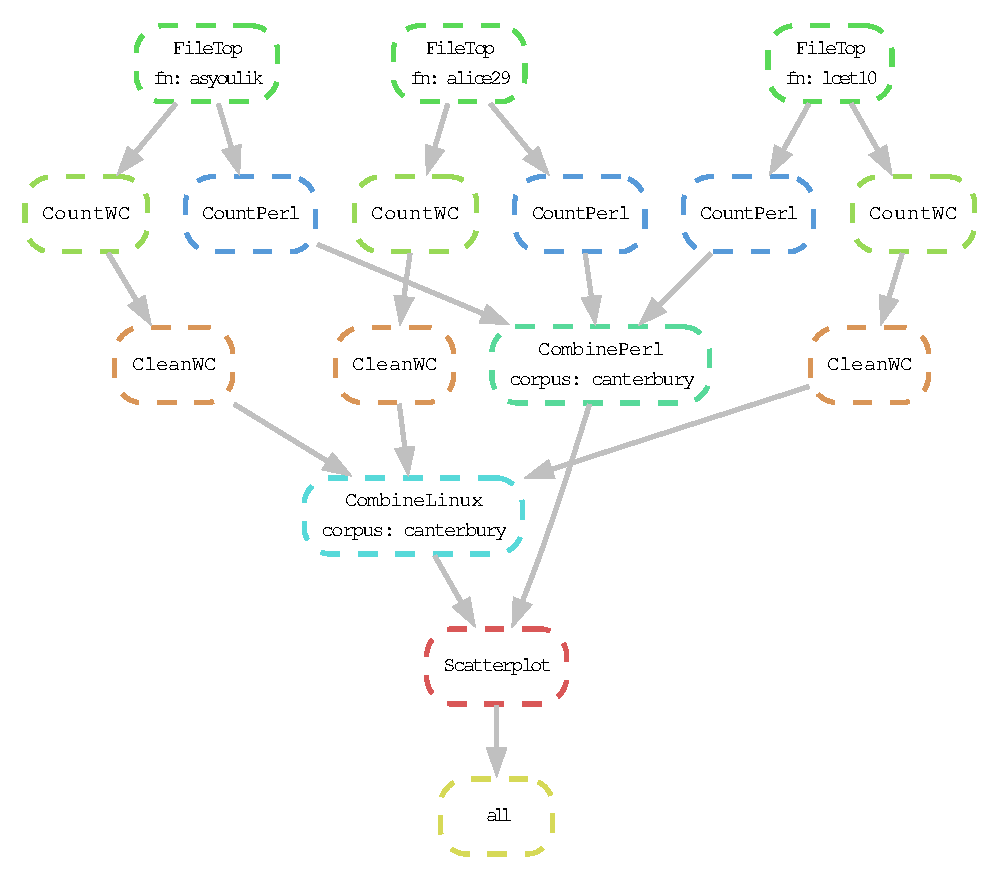
\includegraphics[width=9cm]{finalex/dag-v6}}}
\end{figure}

\end{frame}


%%%%%%%%%%%%%%%%%%%%%%%%%%%%%%%%%%%%%%%%%%%%%%%%%%%%%%%
\begin{frame}[fragile]

\frametitle{Update the all rule}

This can also be done to the {\magenta{all}} rule to process both corpora:
\begin{tiny}
\begin{lstlisting}[frame=single,language=bash]
rule all:
  input:
    OUTPUT_DIR + "/05-graphs/canterbury.jpg",
    OUTPUT_DIR + "/05-graphs/calgary.jpg"
\end{lstlisting}
\end{tiny}

\end{frame}


%%%%%%%%%%%%%%%%%%%%%%%%%%%%%%%%%%%%%%%%%%%%%%%%%%%%%%%
\begin{frame}[fragile]

\frametitle{Some things to note}

\begin{tiny}
\begin{lstlisting}[frame=single,language=bash]
rule Scatterplot:
  input:
    input_fn1 = OUTPUT_DIR + "/04-combine-perl/{corpus}.tsv",
    input_fn2 = OUTPUT_DIR + "/04-combine-linux/{corpus}.tsv",
  output:
    output_fn1 = OUTPUT_DIR + "/05-graphs/{corpus}.jpg",
    output_fn2 = OUTPUT_DIR + "/05-graphs/{corpus}.png",
    output_fn3 = OUTPUT_DIR + "/05-graphs/{corpus}.eps"
  params:
    corpus = "{corpus}",
    myeps = lambda wildcards: config["my_options"]["postscript"]
  log:
    log_fn1 = OUTPUT_DIR + "/05-graphs/{corpus}.log"
  shell:
    """
    ##  {params.corpus} is available
    mypng="png"
    {TOOLS_DIR}/scatterplot.R --type jpg --perl {input.input_fn1} --linux
      {input.input_fn2} --output {output.output_fn1} >{log.log_fn1} 2>&1
    {TOOLS_DIR}/scatterplot.R --type ${{mypng}} --perl {input.input_fn1} --linux
      {input.input_fn2} --output {output.output_fn2} >>{log.log_fn1} 2>&1
    {TOOLS_DIR}/scatterplot.R --type {params.myeps} --perl {input.input_fn1} --linux
      {input.input_fn2} --output {output.output_fn3} >>{log.log_fn1} 2>&1
    """
\end{lstlisting}
\end{tiny}

\end{frame}


%%%%%%%%%%%%%%%%%%%%%%%%%%%%%%%%%%%%%%%%%%%%%%%%%%%%%%%
\begin{frame}

\frametitle{Some things to note}

\begin{itemize}
  \item R script is meant to run on the command-line with supplied arguments (i.e., not interactively in RStudio).
  \item There is a {\blue{log file}}!  If a rule fails, Snakemake deletes all output generated (i.e., in the output directive).  Those sent to the log directive are {\red{not}}.  Looking at them will save you many headaches.
  \item I have given {\green{names}} to the input, output, and log directives.  Without names and as a list, you can also refer to files with an index:  {\texttt{input[2]}} (i.e., the third file in the input directive)
\end{itemize}

\end{frame}


%%%%%%%%%%%%%%%%%%%%%%%%%%%%%%%%%%%%%%%%%%%%%%%%%%%%%%%
\begin{frame}[fragile]

\frametitle{Some things to note}

From {\texttt{config.yml}}:
\begin{tiny}
\begin{lstlisting}[frame=single,language=bash]
fileslist:  "fileslist.tsv"

my_options:
  postscript:  "eps"
\end{lstlisting}
\end{tiny}

\begin{itemize}
  \item Note 3 ways the argument to {\texttt{--type}} is provided and used:
  \begin{enumerate}
    \item {\texttt{jpg}} as literal text
    \item {\texttt{png}} as a bash variable
    \item {\texttt{eps}} as a Snakemake variable which is stored in a file called {\texttt{config.yml}}.  Note the use of {\texttt{lambda}} to access the dictionary created by the configuration file.
  \end{enumerate}
\end{itemize}

\end{frame}


%%%%%%%%%%%%%%%%%%%%%%%%%%%%%%%%%%%%%%%%%%%%%%%%%%%%%%%
\begin{frame}

\frametitle{Much larger Snakemake example}

\begin{figure}
  \centering
  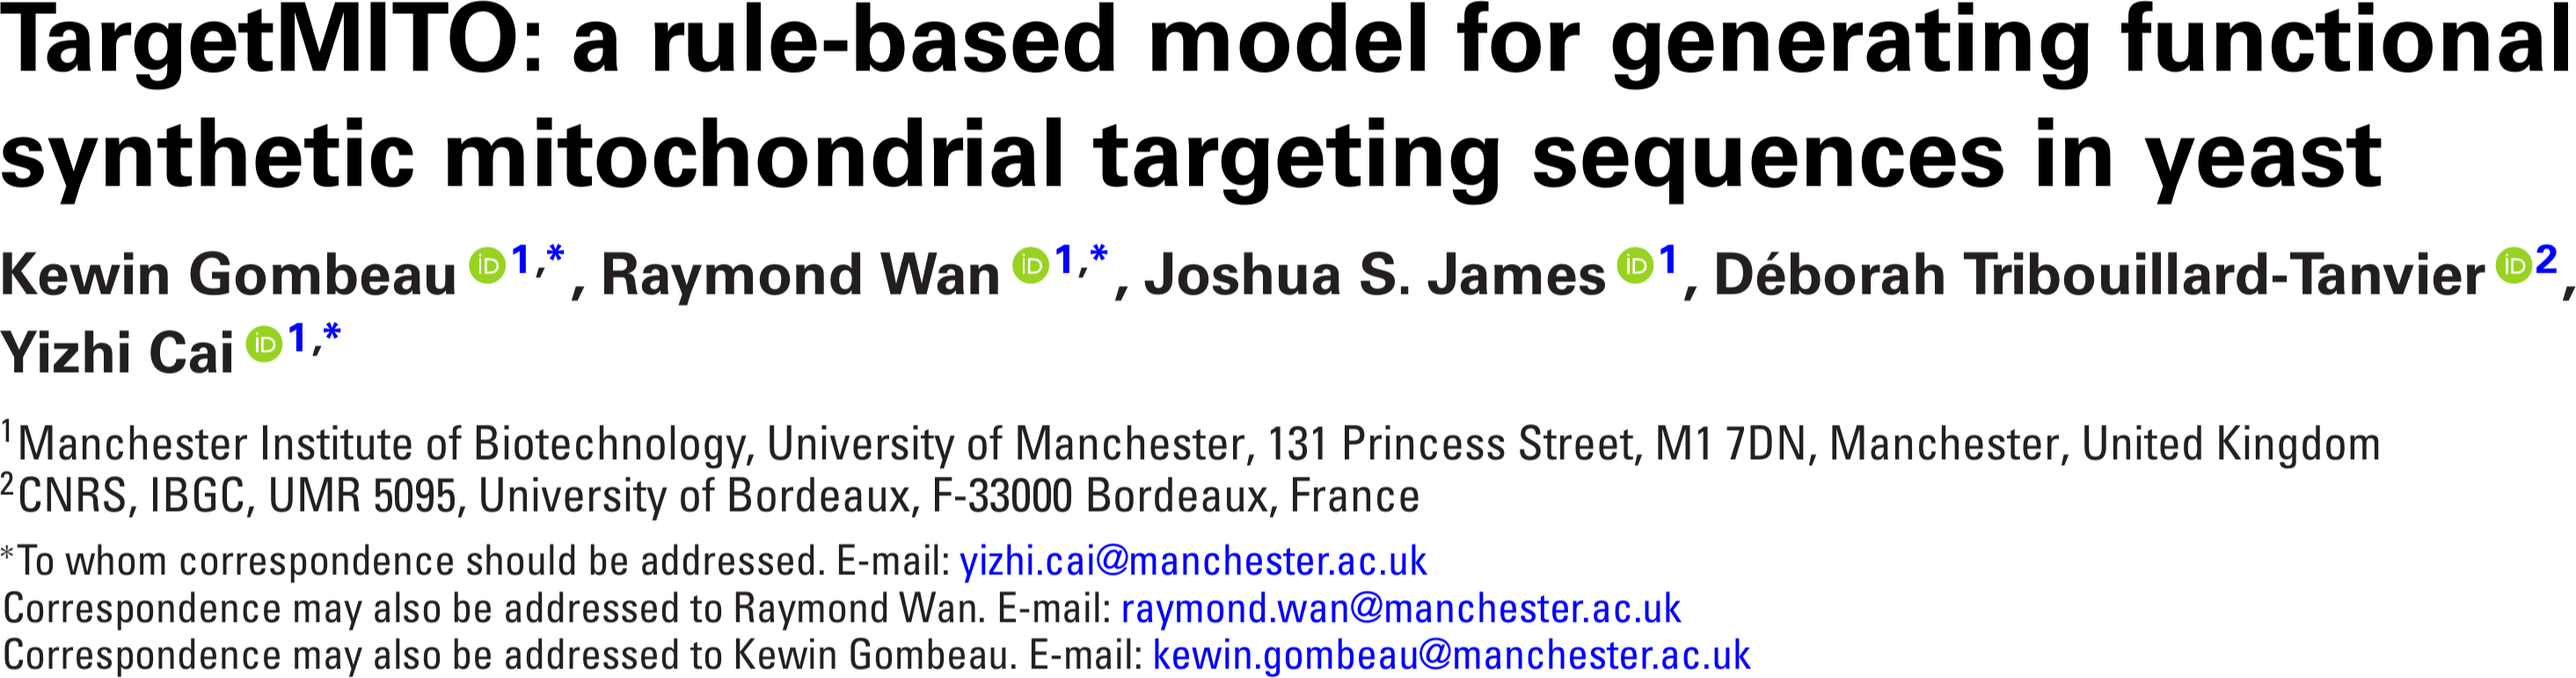
\includegraphics[width=\linewidth]{structure/gwjtc26-nar}
\end{figure}

\end{frame}


%%%%%%%%%%%%%%%%%%%%%%%%%%%%%%%%%%%%%%%%%%%%%%%%%%%%%%%
\begin{frame}

\frametitle{Larger Snakemake example}

GitHub repository (\href{https://github.com/the-cai-lab/synMTS}{https://github.com/the-cai-lab/synMTS}) has 4 workflows meant to run in order:

\begin{enumerate}
  \item generate -- Generate synthetic mitochondria targeting sequences (synMTS)
  \item evaluate -- Evaluate these sequences
  \item statistics -- Calculate some statistics over the properties of the synMTS
  \item select -- Take a subset of the results to focus on [for the manuscript]
\end{enumerate}

\end{frame}





%%%%%%%%%%%%%%%%%%%%%%%%%%%%%%%%%%%%%%%%%%%%%%%%
%%%%%%%%%%%%%%%%%%%%%%%%%%%%%%%%%%%%%%%%%%%%%%%%
\section{Tips}


%%%%%%%%%%%%%%%%%%%%%%%%%%%%%%%%%%%%%%%%%%%%%%%%%%%%%%%
\begin{frame}

\frametitle{Building a workflow}

\begin{enumerate}
  \item I ``looked down'' on {\texttt{bash}} scripts before, but you might want to start from that on one data file first as a starting point.  Convert this to a Snakemake file.
  \item Because of how wildcards are carried backwards (i.e., the {\green{corpus}} variable), you might want to start connecting things up from the {\magenta{all}} rule.
  \item The Linux {\texttt{touch}} command can be useful here.  It updates the date/time or creates a new file with 0 bytes with the current date and time.
    \begin{itemize}
      \item So, you can link up the workflow first with {\texttt{touch \{output\}}} and then write the actual commands afterwards.
    \end{itemize}
  \item I started {\red{numbering}} my output directories to help me figure out the order of the output files.
  \item Send error messages of programs to the {\blue{log}} directive.  If a rule fails, then you have a message to read.
\end{enumerate}

\end{frame}


%%%%%%%%%%%%%%%%%%%%%%%%%%%%%%%%%%%%%%%%%%%%%%%%%%%%%%%
\begin{frame}

\frametitle{Testing a workflow}

Use:
\begin{itemize}
  \item a small test file.
  \item a single core ({\texttt{--cores 1}}) when testing.  With more cores, the rules are executed simultaneously.  Thus, the output will interleave and you can't tell which rule output what!
  \item the {\texttt{-p}} option so that it prints the command that it is running.
\end{itemize}

\end{frame}


%%%%%%%%%%%%%%%%%%%%%%%%%%%%%%%%%%%%%%%%%%%%%%%%%%%%%%%
\begin{frame}

\frametitle{Debugging a workflow}

\begin{figure}
  \centering
  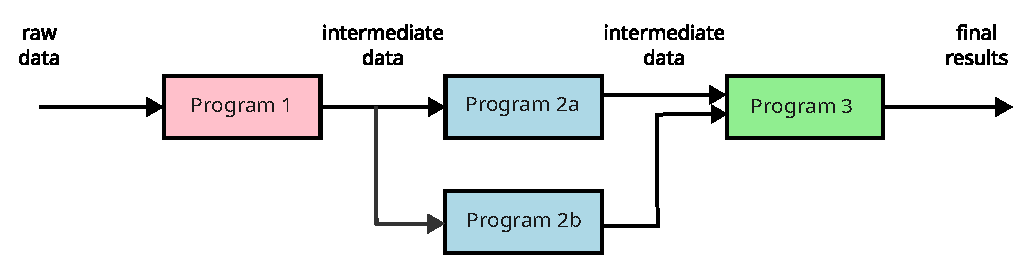
\includegraphics[width=\linewidth]{tips/pipeline-example-branching.eps}
\end{figure}

When trying to find out where in your workflow is causing you grief, you can remove an entire branch by commenting it out from the {\green{input}} directive of the rule it is going to.
\vs

Snakemake seems to:
\begin{enumerate}
  \item Start from the end to the beginning, looking for which paths to follow.
  \item When the execution paths are known, it runs it in the forward direction from the beginning.
\end{enumerate}

\end{frame}


%%%%%%%%%%%%%%%%%%%%%%%%%%%%%%%%%%%%%%%%%%%%%%%%%%%%%%%
\begin{frame}

\frametitle{Common error message}

\begin{figure}
{\fbox{
  \begin{tabularx}{\linewidth}{X}
IncompleteFilesException:\\
The files below seem to be incomplete. If you are sure that certain files are not incomplete, mark them as complete with\\
\\
{\D\D}snakemake --cleanup-metadata <filenames>\\
\\
To re-generate the files rerun your command with the --rerun-incomplete flag.  Incomplete files:\\
...\\
\end{tabularx}
}}
\end{figure}
\vs

Snakemake stores its progress in a run in a ``hidden'' directory called {\red{\texttt{.snakemake}}}.  If it starts getting its state wrong (i.e., you think it completed its last run, but it does not think so), then delete this directory and all of the output.  Then, start again.

\end{frame}



%%%%%%%%%%%%%%%%%%%%%%%%%%%%%%%%%%%%%%%%%%%%%%%%
%%%%%%%%%%%%%%%%%%%%%%%%%%%%%%%%%%%%%%%%%%%%%%%%
\section{Summary}


%%%%%%%%%%%%%%%%%%%%%%%%%%%%%%%%%%%%%%%%%%%%%%%%%%%
\begin{frame}

\frametitle{GitHub repository}

\dirtree{%
.1 .
.2 \myfolder{green}{data}\DTcomment{Data files}.
.3 \myfolder{green}{calgary}\DTcomment{Part of the Calgary corpus}.
.3 \myfolder{green}{canterbury}\DTcomment{Part of the Canterbury corpus}.
.2 \myfolder{red}{slides}\DTcomment{\LaTeX source of these slides}.
.2 src\DTcomment{All of the examples}.
.3 \myfolder{blue}{tools}\DTcomment{Perl and R scripts used}.
.3 \myfolder{blue}{v1}\DTcomment{Makefile example}.
.3 \myfolder{blue}{v2}\DTcomment{Single rule}.
.3 \myfolder{blue}{v3}\DTcomment{Two rules}.
.3 \myfolder{blue}{v4}\DTcomment{Generalisation}.
.3 \myfolder{blue}{v5}\DTcomment{Python in a run directive}.
.3 \myfolder{blue}{v6}\DTcomment{Final, largest example}.
}

The PDF of the slides are at the top directory.

\end{frame}


%%%%%%%%%%%%%%%%%%%%%%%%%%%%%%%%%%%%%%%%%%%%%%%%%%%
\begin{frame}

\frametitle{Snakemake $=$ Python}

{\red{$\rightarrow$}} Not really...
\vs

Since the developers made Snakemake with Python, there are many opportunities to leverage Python.
\begin{itemize}
  \item A Python function to return a list of inputs paths.
  \item A {\texttt{run}} directive (or {\texttt{script}} directive) that accepts Python code.
\end{itemize}
\vs

But, you can write a Snakemake workflow without calling any Python code.

\end{frame}


%%%%%%%%%%%%%%%%%%%%%%%%%%%%%%%%%%%%%%%%%%%%%%%%%%%
\begin{frame}

\frametitle{Snakemake $=$ ``reproducibility''}

{\red{$\rightarrow$}} Unfortunately, no...
\vs

We are all looking for that ``magical'' method.  If this method is used, then reproducibility of our analysis is ``guaranteed''.
\vs

Snakemake {\red{is}} a step in the right direction.  But using it alone does not guarantee reproducibility.

\end{frame}


%%%%%%%%%%%%%%%%%%%%%%%%%%%%%%%%%%%%%%%%%%%%%%%%%%%
\begin{frame}

\frametitle{Analogy}

Snakemake defines a workflow, which is analogous to a recipe for baking.  If you follow it, you will get the same cake every time.
\vs

But suppose the recipe asks for whole milk and, for whatever reason, whole milk is no longer available anywhere.  You will need to substitute it with skim milk or oat milk (for example).  Even if you still use the same quantity as the recipe, the end result will not be the same.
\vs

Something outside of the recipe (and beyond your control) has made reproducibility not possible.

\end{frame}


%%%%%%%%%%%%%%%%%%%%%%%%%%%%%%%%%%%%%%%%%%%%%%%%%%%
\begin{frame}[fragile]

\frametitle{More concrete example}

This appears in one of the Perl scripts today:

\begin{tiny}
\begin{lstlisting}[frame=single,language=perl]
use AppConfig;
use AppConfig::Getopt;
\end{lstlisting}
\end{tiny}

It allows a Perl script to process arguments on the command-line.  On my system, version 1.71-2.3build1 of AppConfig was used.  Years later, this version might be too old and version 2.00 (for example) might be needed.
\vs

There are ways to {\magenta{lock}} (or pin) libraries down to an exact version to address this problem.  But if the system administrator tells you that version 1.71-2.3build1 has a serious security flaw and ``you must upgrade'' or ``you will not be allowed to run it'', then you have no choice. 

\end{frame}


%%%%%%%%%%%%%%%%%%%%%%%%%%%%%%%%%%%%%%%%%%%%%%%%%%%
\begin{frame}

\frametitle{Support of Jupyter notebooks?}

{\red{$\rightarrow$}} Unfortunately, no...
\vs

I am not an expert on Jupyter notebooks, but they seem to be very good at {\green{interactive}} analysis of data.  Similar to RStudio.
\vs

With Snakemake, you need to write scripts (i.e., Python, R, etc.) that are not interactive.  Parameters can be supplied to affect how the program is run.

\end{frame}


%%%%%%%%%%%%%%%%%%%%%%%%%%%%%%%%%%%%%%%%%%%%%%%%%%%
\begin{frame}

\frametitle{Support for SLURM/CSF3?}

{\red{$\rightarrow$}} Yes!
\vs

Over 5 years ago, I created Snakemake scripts that would send $x$ (which you specify) jobs to SLURM.  As your my jobs completed, new ones are added so that there are always around $x$ jobs running / queued.
\vs

Looking at the documentation, the method to do this appears to have changed.  Now, it might called {\href{https://snakemake.readthedocs.io/en/v9.18.1/executing/executors.html}{{\red{executors}}}}.
\vs

The problem for CSF3 is that you need your Snakemake script to be {\magenta{continuously}} running on the login node.

\end{frame}


%%%%%%%%%%%%%%%%%%%%%%%%%%%%%%%%%%%%%%%%%%%%%%%%%%%
\begin{frame}

\frametitle{Support for SLURM/CSF3}

E-mail from September 2026:
\begin{figure}
  \centering
  {\fbox{
\includegraphics[width=\linewidth]{summary/csf3}}}
\end{figure}

Link in message:  \href{https://ri.itservices.manchester.ac.uk/csf3/software/applications/nextflow/}{https://ri.itservices.manchester.ac.uk/csf3/software/applications/nextflow/}

\end{frame}


%%%%%%%%%%%%%%%%%%%%%%%%%%%%%%%%%%%%%%%%%%%%%%%%%%%
\begin{frame}

\frametitle{Summary}

\begin{itemize}
  \item If you're using {\texttt{bash}} scripts or copy-and-pasting commands in from a lab notebook for a workflow consisting of many steps, you should consider some workflow-based system.
  \item Snakemake is one of many options.
  \item Of course, if you only run only a few commands, then Snakemake might be more than what you need!
\end{itemize}

\end{frame}





%%%%%%%%%%%%%%%%%%%%%%%%%%%%%%%%%%%%%%%%%%%%%%%%%%%
\begin{frame}

\frametitle{Acknowledgements}

\begin{itemize}
  \item \LaTeX\  template for these slides due to {\href{https://github.com/Non-Invasive-Bioelectronics-Lab/uom_beamer_template}{Alex Casson}}, which in turn is due to \href{https://github.com/mundya/unofficial-university-of-manchester-beamer}{Andrew Mundy}.
  \item QR code generation due to Adobe Express \href{https://www.adobe.com/express/feature/image/qr-code-generator}{web site}.
  \item Image generation / conversion:  Gimp and Inkscape.
  \item Test data files:  Calgary corpus \citep{bcw90:book} and Canterbury corpus \citep{ab97:dcc}.  Both were obtained from \href{https://corpus.canterbury.ac.nz/}{https://corpus.canterbury.ac.nz/}.
\end{itemize}

\end{frame}


%%%%%%%%%%%%%%%%%%%%%%%%%%%%%%%%%%%%%%%%%%%%%%%%%%%
\begin{frame}

\frametitle{Questions?}

\begin{center}
E-mail:  \href{mailto:raymond.wan@manchester.ac.uk}{raymond.wan@manchester.ac.uk}
\end{center}

Computational Biology at Manchester Teams; Scripting and Coding channel:
\begin{figure}
  \centering
  
\includegraphics[height=5cm]{qrcodes/teams-scripts}
\end{figure}

\end{frame}


%%%%%%%%%%%%%%%%%%%%%%%%%%%%%%%%%%%%%%%%%%%%%%%%%%%
\begin{frame}

\frametitle{Questions?}

\begin{figure}
  \centering
  \begin{tabular}{cc}
    
\includegraphics[height=5cm]{qrcodes/github} &
    
\includegraphics[height=5cm]{qrcodes/nar} \\
    These slides & NAR paper \\
  \end{tabular}
\end{figure}

\end{frame}


%%%%%%%%%%%%%%%%%%%%%%%%%%%%%%%%%%%%%%%%%%%%%%%%%%%
\begin{frame}[allowframebreaks]

\frametitle{References}

\printbibliography

\end{frame}


\end{document}


